% Select one class
%\documentclass{pucthesis}		% For DVI
\documentclass[pdftex]{pucthesis}	% For pdfLaTeX
%\documentclass[spanish]{pucthesis}		% For DVI, in spanish
%\documentclass[pdftex,spanish]{pucthesis}	% For pdfLaTeX, in spanish

%%%%%%%%%
%   Packages	 %
%%%%%%%%%

% Floats
\usepackage{graphicx}
\usepackage{float}
% \floatstyle{boxed}
\restylefloat{figure}
\usepackage{color}
\usepackage{caption}
\usepackage{subcaption}
\usepackage{varwidth}

% Math packages
\usepackage{amsmath}
\usepackage{amsfonts}
\usepackage{amssymb}
\usepackage{stmaryrd}
\usepackage{mathtools}
\usepackage{algorithm}
\usepackage[noend]{algpseudocode}

% Closest font to Times New Roman
\usepackage{mathptmx}

% To make pretty tables
\usepackage{booktabs}
\usepackage{multirow}

% To avoid underfull errors in the bibliography
\usepackage{etoolbox}
\apptocmd{\sloppy}{\hbadness 10000\relax}{}{}

% To make cites and references
\usepackage[hidelinks,pdfusetitle,pdfdisplaydoctitle]{hyperref}
\usepackage[natbibapa]{apacite} 
\usepackage{doi}
\renewcommand{\doitext}{}

% TiKZ
\usepackage{tikz}
\usetikzlibrary{automata,graphs,positioning,fit,backgrounds,chains,arrows,decorations.pathmorphing,decorations.pathreplacing,calc}

\input{sources/ecs.tikzstyles}

%--------- NEW ENVIRONMENTS --------- You are free to remove or use it
\newtheorem{definition}{\bf Definition}[chapter]
\newtheorem{property}{Property}[chapter]
\newtheorem{claim}{Claim}[chapter]
\newtheorem{lemma}{\bf Lemma}[chapter]
\newtheorem{proposition}{Proposition}[chapter]
\newtheorem{theorem}{\noindent \bf Theorem}[chapter]
\newtheorem{corollary}{\bf Corollary}[chapter]
\newtheorem{pf}{Proof}[chapter]
\newtheorem{example}{\bf Example}[chapter]
\newtheorem{remark}{Remark}[chapter]

% En caso de que el título sea muy largo, se puede ajustar el espacio
% antes y después de este en las dos primeras páginas para que quede centrado.

%\makeatletter
%  \setlength{\beftitle}{105\p@\@plus24\p@}
%  \setlength{\afttitle}{65\p@}
%\makeatother
%%%%%%%%%%%%%%%%%%%%%%%%
%% Complexity classes %%
%%%%%%%%%%%%%%%%%%%%%%%%

\newcommand{\PTIME}{\textnormal{\textsf{PTIME}}}
\newcommand{\EXPTIME}{\textnormal{\textsf{EXPTIME}}}
\newcommand{\TWOEXPTIME}{\textnormal{\textsf{2EXPTIME}}}
\newcommand{\PSPACE}{\textnormal{\textsf{PSPACE}}}
\newcommand{\EXPSPACE}{\textnormal{\textsf{EXPSPACE}}}
\newcommand{\NPSPACE}{\textnormal{\textsf{NPSPACE}}}
\newcommand{\LOGSPACE}{\textnormal{\textsf{LOGSPACE}}}
\newcommand{\ALOGSPACE}{\textnormal{\textsf{ALOGSPACE}}}
\newcommand{\NLOGSPACE}{\textnormal{\textsf{NLOGSPACE}}}
\newcommand{\coNLOGSPACE}{\textnormal{\textsf{coNLOGSPACE}}}
\newcommand{\NP}{\textnormal{\textsf{NP}}}
\newcommand{\coNP}{\textnormal{\textsf{coNP}}}
\newcommand{\FPT}{\textnormal{\textsf{FPT}}}
\newcommand{\pitwop}{\Pi_2^p}

%%%%%%%%%%%%%%%%%%
%% Span-related %%
%%%%%%%%%%%%%%%%%%

\newcommand{\bbN}{\mathbb{N}}
\newcommand{\Span}[2]{[#1, #2\rangle}
\newcommand{\osymbol}{\blacksquare}
\newcommand{\cset}{\operatorname{set}}
\newcommand{\oout}{\operatorname{out}}

\newcommand{\cA}{\mathcal{A}}
\newcommand{\cE}{\mathcal{E}}
\newcommand{\cL}{\mathcal{L}}
\newcommand{\eol}{\rotatebox[origin=l]{180}{\ensuremath\Rsh}}
\newcommand{\bof}{\rotatebox[origin=l]{180}{\ensuremath\Lsh}}
%\newcommand{\nl}{\hookleftarrow}
\newcommand{	\VV}{\mathcal{V}}
\newcommand{	\OO}{\mathcal{O}}
\newcommand{	\CC}{\mathcal{C}}
\newcommand{	\NN}{\mathcal{N}}
\newcommand{	\sub}{\text{span}}
\newcommand{	\doc}{\text{doc}}
\newcommand{	\cont}{\text{str}}
\newcommand{	\var}{\text{var}}
\newcommand{	\ivar}{\text{ivar}}
\newcommand{	\hs}{\hat{\sigma}}
\newcommand{\op}[1]{\langle#1\rangle}
\newcommand{	\name}{\text{name}}
\newcommand{	\dom}{\text{dom}}
\newcommand{\sem}[1]{\llbracket#1\rrbracket}
\newcommand{\semseq}[1]{\llbracket#1\rrbracket^{\operatorname{seq}}}
\newcommand{\sems}[1]{\sem{#1}'}
\newcommand{\semp}[1]{\llceil{#1}\rrfloor}
\newcommand{\semg}[1]{\llbracket #1 \rrbracket_{d}}
\newcommand{\semd}[1]{\sem{#1}_{d}}
\newcommand{\seme}[2]{\sem{#1}_{#2}}
\newcommand{\semsd}[1]{\sems{#1}_{d}}
\newcommand{\sempd}[1]{\semp{#1}_{d}}
\newcommand{\semds}[1]{\sem{#1}_{d, \sigma}}
\newcommand{\semcs}[1]{\sem{#1}_{\CC, \sigma}}
\newcommand{	\first}{\text{first}}
\newcommand{	\last}{\text{last}}

\newcommand{	\rematch}{\textsf{REmatch}}


\newcommand{\trans}[2][]{\raisebox{-1pt}[10pt][0pt]{$\overset{#2}{\underset{^{#1}}{\raisebox{0pt}[3pt][0pt]{$\relbar\mspace{-8mu}\rightarrow$}}}$}}

\newcommand{\longtrans}[2][]{\raisebox{-1pt}[10pt][0pt]{$\overset{#2}{\underset{^{#1}}{\raisebox{0pt}[3pt][0pt]{$\relbar\mspace{-8mu}\longrightarrow$}}}$}}

\newcommand{\VA}{\ensuremath{\mathrm{VA}}}
\newcommand{\EVA}{\ensuremath{\mathrm{eVA}}}
\newcommand{\EVAs}{\ensuremath{\mathrm{eVAs}}}
\newcommand{\sEVA}{\ensuremath{\mathrm{seVA}}}
\newcommand{\fEVA}{\ensuremath{\mathrm{feVA}}}
\newcommand{\dsEVA}{\ensuremath{\mathrm{\text{deterministic }seVA}}}
\newcommand{\dfEVA}{\ensuremath{\mathrm{\text{deterministic }feVA}}}
\newcommand{\fVA}{\ensuremath{\mathrm{fVA}}}
\newcommand{\sVA}{\ensuremath{\mathrm{sVA}}}





\newcommand{\mtt}[1]{\mathtt{#1}}

\DeclareMathOperator{\pruns}{\textit{part-runs}}
\DeclareMathOperator{\runs}{\textit{runs}}
\DeclareMathOperator{\aruns}{ARuns}

\newcommand{\SRE}{\ensuremath{\mathrm{SRE}}}
\newcommand{\kSRE}{\ensuremath{\mathrm{kSRE}}}
\newcommand{\SREf}{\ensuremath{\mathrm{SREf}}}
\newcommand{\RGX}{\ensuremath{\mathrm{RGX}}}
\newcommand{\fRGX}{\ensuremath{\mathrm{funcRGX}}}
\newcommand{\fSRGX}{\ensuremath{\mathrm{funcRGX}}}
\newcommand{\SRGX}{\ensuremath{\mathrm{spanRGX}}}
\newcommand{\seqRGX}{\ensuremath{\mathrm{seqRGX}}}
\newcommand{\GRGX}{\ensuremath{\mathrm{GRGX}}}
\newcommand{\kRGX}{\ensuremath{\mathrm{kRGX}}}
\newcommand{\Treelike}{\emph{tree-like}}
\newcommand{\Vars}{\mathcal{V}}
\newcommand{\Annots}{\Gamma}

\newcommand{\Semantic}[1]{\llbracket#1\rrbracket}
\newcommand{\Language}[1]{\mathcal{L}(#1)}
\newcommand{\Var}{\operatorname{var}}
\newcommand{\Succ}{succ}

\newcommand{\Open}[1]{[ #1}
\newcommand{\OpenSmall}[1]{#1~\ ~\mkern-10mu\vdash}
\newcommand{\Close}[1]{#1 \rangle}

\newcommand{\ENUM}{\text{\sc Eval}}

\newcommand{\eval}{\text{\sc Ann}}
\newcommand{\memb}{\text{\sc Memb}}
\newcommand{\nemp}{\text{\sc NonEmp}}
\newcommand{\mdcheck}{\text{\sc ModelCheck}}
\newcommand{\EVAL}{\text{\sc Eval}}
\newcommand{\COUNT}{\text{\sc Count}}
\newcommand{\sat}{\text{\sc Sat}}
\newcommand{\containment}{\text{\sc Containment}}
\newcommand{\iequiv}{\text{\sc InstEquiv}}
\newcommand{\eequiv}{\text{\sc Equiv}}
\newcommand{\isd}{\text{isDoc}}
\newcommand{\cstring}[1]{\vdash\!#1\!\dashv}
\newcommand{\LL}{{\mathcal L}}
\newcommand{\PP}{{\mathcal P}}
\newcommand{\sre}{{\mathcal SRE}}
\newcommand{\nee}{{\mathcal NE}}
\newcommand{\ap}{{\mathcal AP}}
\newcommand{\nap}{{\mathcal NVP}}

\newcommand{\mi}[1]{\text{\it #1}}
\newcommand{\spa}{\text{\textvisiblespace}}

\DeclareMathOperator{\Perm}{Perm}
\DeclareMathOperator{\Op}{Op}

% To fix an error when using references in the title of sections.
\newcommand{\secref}[1]{\lowercase{\ref{#1}}}

%Ref-word up notation:
\newcommand{\rr}{{\bf{r}}}
\newcommand{\SG}{{\bf{\Sigma}}}
\newcommand{\clr}{{\textsc{clr}}}

\DeclareMathOperator{\out}{\textit{out}}
\DeclareMathOperator{\pout}{\textit{part-out}}

\newcommand{\resultlist}{\operatorname{\textit{resultList}}}
\newcommand{\plist}{\operatorname{\textit{list}}}
\newcommand{\plistold}{\plist^{\operatorname{\textit{old}}}}


\renewcommand{\dag}{{DAG}\xspace}
\newcommand{\dags}{{DAGs}\xspace}

\newcommand{\pfirst}{\operatorname{first}}
\newcommand{\plast}{\operatorname{last}}
\newcommand{\pfirsto}{\pfirst^{\operatorname{old}}}
\newcommand{\plasto}{\plast^{\operatorname{old}}}
\newcommand{\newnode}{\operatorname{node}}
\newcommand{\newmap}{\operatorname{map}}
\newcommand{\markers}{\operatorname{Markers}}

\newcommand{\cbot}{\bot}

\newcommand{\cextend}{\texttt{extend}}
\newcommand{\cunion}{\texttt{union}}
\newcommand{\cenumerate}{\texttt{enumerate}}
\newcommand{\ctable}{\operatorname{T}}
\newcommand{\ckeys}{\operatorname{keys}}

\newcommand{\odet}{{\operatorname{det}}}
\newcommand{\mdetnext}{\texttt{next}}

\newcommand{\cdet}{\mathtt{DET}}
\newcommand{\cgarbagecollector}{\mathtt{GarbageCollector}}
\newcommand{\ds}{\mathtt{NM}}
\newcommand{\cinit}{\texttt{emptyNode}}
\newcommand{\coid}{\mathtt{n}}
\newcommand{\citer}{\texttt{phase}}
\newcommand{\cstateslists}{\textsf{setslist}}
\newcommand{\cstateslistss}{\textsf{setslists}}

\let\oldReturn\Return
\renewcommand{\Return}{\State\oldReturn}

\newcommand{\cAoff}{\cA_{\texttt{offset}}}
\newcommand{\sspan}[1]{[#1\rangle}


%%%%%%%%%%%%%%%%%%%%%
%% Figure Commands %%
%%%%%%%%%%%%%%%%%%%%%

\newcommand{\spanNode}[2]{\node[outer sep=0mm, inner sep=10mm,text height=2mm] (l#1)at (0,0) {\Large \texttt{#2}\vphantom{y}};
	\node[node distance=3.5mm,below of=l#1] {\tiny \texttt{#1}};}
\newcommand{\spanNodeP}[3]{\node[outer sep=0mm, inner sep=10mm, right of=l#1, node distance=4mm, text height=2mm, text centered] (l#2) {\Large \texttt{#3}\vphantom{y}};
	\node[node distance=3.5mm,below of=l#2] {\tiny  \texttt{#2}};}


\newcommand\Vtextvisiblespace[1][.3em]{%
	\mbox{\kern.06em\vrule height.3ex}%
	\vbox{\hrule width#1}%
	\hbox{\vrule height.3ex}}

\hyphenpenalty 1000

\begin{document}

\mdate{Month Day, Year}                         % date manuscript changed
\version{1}                                     % manuscript version #

\title[REmatch: a novel regex engine for finding all matches]
{\bf REmatch: a novel regex engine for finding all matches}
\author[Nicolás Andre Van Sint Jan Campos]{Nicolás Andre Van Sint Jan Campos}

\address{Escuela de Ingeniería\\
Pontificia Universidad Católica de Chile\\
Vicuña Mackenna 4860\\
Santiago, Chile\\
{\it Tel.\/} : 56 (2) 354-2000}
\email{nicovsj@uc.cl}

\facultyto                          {the School of Engineering}
%\department   {}
\faculty                            {Faculty of Engineering}
\degree                             {Master of Science in Engineering} 
\advisor                            {Cristian Riveros}
\committeememberA                   {Domagoj Vrgoc}
\guestmemberA                       {Gonzalo Navarro}
\ogrsmember                         {Cristián Tejos}
\subject                            {Computer Science}
\date                               {October 2023}
\copyrightname                      {Nicolás Van Sint Jan}
\copyrightyear                      {MMXXIII}
\dedication                         {To my parents, Franz and Daniela.}

%%%%%%%%%%%%%%%%%%%%
%       PRELIMINARIES                              %
%----------------------------------------------------%
%      page i & ii: cover page                   %
%      page iii: dedication                         %
%%%%%%%%%%%%%%%%%%%%

\NoChapterPageNumber
\fancyhf{}
\fancyfoot[C]{\fontsize{11pt}{11pt}\selectfont\thepage}
\pagenumbering{roman}
\maketitle
\topmargin -20mm
\headheight 7mm
\headsep 20mm
\oddsidemargin 7.3mm

%%%%%%%%%%%%%%%%%%%%
%   EXTRA PAGES                                     %
%----------------------------------------------------%
%      page --: not used                             %
%%%%%%%%%%%%%%%%%%%%

%\newpage
%\thispagestyle{empty}

%----------------------------------------------------------------------%


%%%%%%%%%%%%%%%%%%%%%%%%%
%      page v: ACKNOWLEDGEMENTS                   %
%%%%%%%%%%%%%%%%%%%%%%%%%

\phantomsection \label{acknowledgements} % Comment if hyperref is unused
\chapter*{ACKNOWLEDGEMENTS}
Write in a sober style your acknowledgements to those persons that contributed to the development and preparation of your thesis.



\cleardoublepage

%----------------------------------------------------------------------%

%%%%%%%%%%%%%%%%%%
%          page v & up ---                      %
%            Table of contents              %
%            List of figures                     %
%            List of tables                      %
%%%%%%%%%%%%%%%%%%

\pdfbookmark{\contentsname}{toc}
\tableofcontents
\phantomsection \label{listoffigures}
\listoffigures
\phantomsection \label{listoftables}
\listoftables
\cleardoublepage

%----------------------------------------------------------------------%

%%%%%%%%%%%%%%%%%%%%%%%%
%      page x & xi: ABSTRACT - RESUMEN        %
%%%%%%%%%%%%%%%%%%%%%%%%

\phantomsection \label{abstract}
\chapter*{ABSTRACT}
In this thesis, we present the \rematch\ system for information extraction. \rematch\ is based on a recently proposed enumeration algorithm for evaluating regular expressions with capture variables supporting the all-match semantics. It tells a story of what it takes to make a theoretically optimal algorithm work in practice. As we show here, a naive implementation of the original algorithm would have a hard time dealing with realistic workloads. We thus develop a new algorithm and a series of optimizations that make \rematch\ as fast or faster than many popular RegEx engines while at the same time being able to return all the outputs: a task that most other engines tend to struggle with. \

\vfill
\noindent {\bf Keywords}:  regular expressions, document spanners, information extraction, enumeration algorithms, all-match semantics.

\cleardoublepage

\phantomsection \label{resumen}
\chapter*{RESUMEN}
El resumen debe contener entre 100 y 300 palabras. El resumen debe ser escrito en ingl\'es y espa\~nol.  En el caso de tesis de doctorado, el formato de la p\'agina del resumen es distinta, por favor verifique la plantilla entregada por la Direcci\'on de Postrgrado.\

\vfill
\noindent {\bf Palabras Claves}: plantilla de tesis, escritura de documentos, {\bf (Colocar aqu\'i las palabras claves relevantes y estr\'ictamente relacionadas al tema de la tesis)}.

\cleardoublepage

%%%%%%%%%%%%%
%   TEXT  OF THESIS     %
%%%%%%%%%%%%%

\pagenumbering{arabic}

\chapter[INTRODUCTION]{Introduction}
% % !TeX root = ../main.tex

Regular expressions, or RegEx, are one of the most used technologies for managing text data. The development of RegEx engines started in the early 70s~\cite{thompson1968programming,earlyNFA}, and they are now a common part of many complex information systems such as compilers, databases, or search engines. Moreover, modern RegEx engines are highly-optimized systems that are crucial for finding patterns in diverse areas like biology~\cite{Gonzalo}, literature~\cite{lit1}, or medicine~\cite{FloresFP21}. 


Given a regular expression and a document, the task of a RegEx engine is to find all occurrences, or \emph{matches}, of the pattern in the document. For this, RegEx engines deploy the so-called \emph{leftmost-longest} paradigm~\cite{posix}, meaning that they find the match which is the leftmost one, and from there they find the longest possible match. The process is then repeated  starting from the rightmost position of the previous match\footnote{Although RegEx engines follow different matching rules, the leftmost-longest rule is at the core of most modern engines. For a detailed discussion see \cite{friedl2006mastering}.}. For example, if we want to evaluate the RegEx $\texttt{aa}$ over the document $a_0 a_1 a_2 a_3$ (here the subindices are for referencing positions; the document consists of the letter $a$ repeated four times), a typical RegEx engine will output the matches $a_0a_1$ and $a_2a_3$. In particular, RegEx engines will not output $a_1a_2$ since the first leftmost-longest match ends with $a_1$. 

The leftmost-longest semantics is standard for  RegEx engines, as it captures the majority of meaningful matches, although not all of them. However, in some scenarios adopting an ``all-match semantics'' is a valuable and desirable feature for the users. For instance, in DNA analysis we will often need to match patterns (called motifs) onto a DNA sequence, and these can overlap. The question of finding overlapping matches with RegEx is also recurrent in user discussions~\cite{overlap1,overlap2,overlap3}. For information extraction, the all-match semantics leaves freedom to the user to extract all positions, called spans, where there is relevant information in a document. Therefore the all-match semantics is a desirable feature for RegEx engines that, to the best of our knowledge, no engine supports natively.

To overcome the problem of finding all-matches, RegEx engines offer look-around operators, namely, operators that allows checking if a subexpression can be matched forward or backward from the current position, without advancing from the current position. For instance, by using look-around, we can modify the expression \texttt{aa} to \texttt{(?=(aa))} and find the missing match $a_1a_2$ over the above document. Despite this example, look-around operators cannot discover all matches for every RegEx expression. For instance, given the look-around definition, one cannot extract two matches that start at the same position (for concrete examples see Section~\ref{chpt:regex} and Section~\ref{sec:experiments}).

In terms of implementation, RegEx engines are usually divided into three categories: DFA-based, NFA-based, and recursive NFA-based~\cite{cox2007regular}. DFA is generally the fastest evaluation strategy, followed by (plain) NFA. In contrast, recursive NFA-based engines use backtracking, which is susceptible to well-documented performance issues, like regular expression denial of service attacks (ReDos)~\cite{friedl2006mastering}, where the engine can exhibit exponential time performance~\cite{cox2007regular}. From the positive side, recursive NFA-based engines have the advantage of keeping track of the evaluation, which allows implementing operators like look-around and back-references.
In summary, until now, the only way of finding all matches (in some cases) is by using look-around operators implemented by recursive NFA-based engines, which suffer from unfortunate performance issues. 

To overcome these issues, this thesis presents \rematch, a RegEx engine supporting the all-match semantics, and its accompanying regular expression language REQL. Contrary to the status quo of RegEx evaluation, \rematch\ is based on a new evaluation strategy, inspired by the theory of enumeration algorithms~\cite{Segoufin13}, that allows finding all the matches, and avoids the exponential behavior of recursive NFA evaluation. Moreover, \rematch\ performance is comparable to popular RegEx engines, while at the same time finding all the matches, thus obtaining the best of both worlds. Specific contributions of the thesis are as follows:

\begin{enumerate}

\item  We introduce the REQL query language, which extends classical RegEx with variables and the all-match semantics.	

\item We present \rematch, a RegEx system whose architecture allows evaluating REQL using output-linear delay. For this, we develop a new evaluation method which extends the theoretical algorithm of~\cite{FlorenzanoRUVV20} and incorporates new optimization techniques, allowing \rematch\ to compete with modern RegEx engines. 

\item We develop a set of experiments to evaluate the effect of different optimizations on \rematch\ performance, and compare it to existing RegEx engines. Although \rematch\ uses a more general semantics, we show that its performance stacks well compared to other engines.
	
\end{enumerate}

In Chapter~\ref{chpt:regex} we introduce REQL. We then explain each module of the \rematch\ architecture (see~Figure~\ref{fig:architecture}). Chapter~\ref{chpt:rewriting} presents the rewriting module, Chapter~\ref{chpt:filtering} the filtering module, and Chapter~\ref{chpt:output} the output module. Chapter~\ref{sec:evaluation} explains the evaluation algorithm of \rematch. Chapter~\ref{sec:experiments} puts all components together and displays the experimental comparison with other engines. We conclude in Chapter~\ref{sec:conclusions} by discussing possible future work. 


\chapter[REQL: A REGEX QUERY LANGUAGE FOR IE]{REQL: a RegEx Query Language for IE} \label{chpt:regex}
% !TeX root = ../main.tex !TeX spellcheck = en_US

This section introduces REQL, a RegEx Query Language for information extraction,
that we implement in \rematch. The language is an extension of the classical
RegEx syntax (e.g. POSIX Basic Regular Expressions) familiar to most users. On
the other hand, the semantics is inspired by the document spanner
framework~\citep{FaginKRV15} that captures all appearances of a pattern in the
document. 

In the following, we present the formal syntax and semantics of REQL, and
provide several examples of REQL queries.

\section{Documents and spans}

We follow the theoretical framework of documents and spans introduced
in~\citep{FaginKRV15}. For us, a document $d$ is simply a string over some finite
alphabet (e.g. the ASCII charset, UTF-8, or a similar encoding
scheme)\footnote{Note that a multi-line document is simply a single string.}. We
write $d = a_0a_1 \ldots a_{n-1}$ to denote a document of length $|d| = n$ where
$a_{i}$ is the $i$-symbol (note that the first symbol starts from
$0$)\footnote{In \citep{FaginKRV15}, the first position is $1$. We use $0$ to be
compliant with programming languages and RegEx engines which use $0$ as the
start position.}. An example of a document is given in Figure~\ref{fig-doc}. A
\emph{span} of a document $d$ (also called a \emph{match}) is a pair $s =
[i,j\rangle$ of natural numbers $i$ and $j$ with $0 \leq i \leq j\leq |d|$. In
that case, $s$ is associated with the continuous region of the document~$d$
whose content is the substring of $d$ from position $i$ to position $j-1$. We
denote this substring by $d(s)$ or $d(i,j)$. For instance, $d_1([0,4\rangle) =
\texttt{that}$, since this is the content of the string $d$ in positions 0
through~3.
%
Notice that if $i = j$, then $d(s) = d(i,j) = \varepsilon$, the empty string.
Given two spans $s_1 = [i_1, j_1\rangle$ and $s_2 = [i_2, j_2\rangle$ such that
$j_1 = i_2$, we define their \emph{concatenation} as $s_1 \cdot s_2=[i_1,
j_2\rangle$. The set of all spans of $d$ is denoted by $\sub(d)$.


\section{Syntax} 
Syntactically, REQL is similar to standard regular expressions, apart from a
special construct \texttt{!x\{e\}}, which states that a substring matching
\texttt{e} should be stored into the variable name \texttt{x}. Formally, the
syntax of REQL queries can be defined as follows:
$$
\begin{array}{rcl}
\texttt{e} & \coloneqq & \texttt{a} \ \mid \ \texttt{.} \ \mid \
\texttt{[w]} \ \mid \ \texttt{[\textasciicircum w]} \ \mid \
%\ \texttt{\textasciicircum} \ \mid \ \texttt{\$}  \\
\texttt{!x\{e\}}  \ \mid \\
& &  \texttt{e} \texttt{e} \ \mid \
\texttt{e|e} \ \mid \ \texttt{e*} \ \mid \ \texttt{e+} \ \mid \ \texttt{e?} \ \mid \ \texttt{e\{n,m\}}
\end{array}
$$
Here, $\texttt{a}$ is a character (e.g., ASCII charset or UTF-8), the dot symbol
is a wildcard for any character, and $\texttt{[w]}$ or
$\texttt{[\textasciicircum w]}$ are a char class or the negation of a char
class, respectively, where $\texttt{w}$ declares a set of characters. We use the
standard notation of ranges of ASCII characters found in POSIX for declaring
char classes (e.g. $\texttt{[a-z]}$, $\texttt{[A-Z0-9apt]}$, etc) and write
$\text{set}(\texttt{w})$ to denote the set of characters represented by
$\texttt{w}$ (e.g. $\text{set}(\texttt{a-z}) = \{a, b, ..., z\}$). Moreover,
$\texttt{x}$ is a variable name where the character \texttt{!} is used to
differentiate a variable name from a letter or string of the alphabet. This,
along with the use of~\texttt{\{} and~\texttt{\}} for delimiting the captured
subregex is the only special notation where we differ from POSIX. Finally,
$\texttt{n}$ and $\texttt{m}$ are numbers such that $0 \leq \texttt{n} \leq
\texttt{m}$. In the REmatch system, REQL also allow the usual regex
abbreviations for character classes (e.g. \texttt{$\backslash$d} for a digit, or
\texttt{$\backslash$w} for a word, etc), however, we do not include them in the
formal definition in order to keep the presentation concise\footnote{We remark
that the start-of-file symbol ($\texttt{\textasciicircum}$) and end-of-file
symbol ($\texttt{\$}$) are currently not supported in \rematch. However, adding
them is a straightforward exercise.}.


\begin{figure}
	\vspace*{-7mm}
	\begin{center}
		%\hspace*{-0.7cm}
		\resizebox{.4\linewidth}{!}{
			\begin{tikzpicture}[baseline=0ex, node distance=1.5cm, every text
				node part/.style={align=center}] \spanNode{0}{t}
				\spanNodeP{0}{1}{h} \spanNodeP{1}{2}{a} \spanNodeP{2}{3}{t}
				\spanNodeP{3}{4}{h} \spanNodeP{4}{5}{a} \spanNodeP{5}{6}{t}
				\spanNodeP{6}{7}{h} \spanNodeP{7}{8}{a} \spanNodeP{8}{9}{t}
				\draw ($(l0) + (-0.1, -0.2)$) to ($(l9) + (0.1, -0.2)$); \node
				at ($(l0) + (-0.6, 0.05)$) {$d_1 :=\ $};
			\end{tikzpicture}
		}
	\end{center}
	\vspace*{-7mm}
	\caption{A sample document for illustration purposes.}
	\label{fig-doc}
\end{figure}



\begin{example}\label{example:basic} To give a preliminary example of how REQL
works, assume that we would like to extract all the occurrences of the word
``that" from a text document. This can be done in REQL as follows:
$$
\texttt{e0} := \texttt{\textbf{!x\{}that\textbf{\}}}
$$
Intuitively, the query captures the positions of a substring \texttt{that} into
the variable $x$. This query also illustrates a key feature of our semantics
(defined below): there can be overlapping matches. To make this more clear,
consider the document $d_1$ in Figure \ref{fig-doc}. The query above will result
in precisely three matches for the variable \texttt{x}, corresponding to the
three occurrences of the substring \texttt{that} in the document we are
processing. The first match will be in positions $[0,4\rangle$, the second in
$[3,7\rangle$, and the last match in $[6,10\rangle$. We notice that the middle
match $[3,7\rangle$ will not be captured by most regular expression tools,
unless some sort of a look-around operator is used.
\end{example}

The reader could notice that the above syntax is so general that one can define
the capture of the same variable multiple times. For instance, a query like
$\texttt{!x\{a!x\{b\}\}}$ defines the capture of $\texttt{x}$ twice. For this
reason, REQL has some simple syntactic restrictions to use variables correctly.
Let $\Var(\texttt{e})$ be the set of all variables names used in $\texttt{e}$.
We say that a REQL query is \emph{well-designed}\footnote{In~\citep{FaginKRV15},
expressions satisfying these conditions are called \emph{functional}.} if every
subquery~$\texttt{e}$ satisfies the following four conditions: (1)~if
$\texttt{e}=\texttt{!x\{e1\}}$, then $\texttt{x} \notin \Var(\texttt{e1})$,
(2)~if $\texttt{e} = \texttt{e1}\,\texttt{e2}$, then
$\Var(\texttt{e1})\cap\Var(\texttt{e2}) = \emptyset$; (3)~if $\texttt{e} =
\texttt{e1}|\texttt{e2}$, then $\Var(\texttt{e1})=\Var(\texttt{e2})$; and (4)~if
$\texttt{e}$ is equal to \texttt{e1*}, \texttt{e1+}, \texttt{e1?} or
\texttt{e1\{n,m\}}, then $\Var(\texttt{e1}) = \emptyset$. One can easily check
that queries $\texttt{!x\{a!x\{b\}\}}$, $\texttt{!x\{a\}!x\{b\}}$,
$\texttt{a|!x\{b\}}$, or $\texttt{(!x\{a\}b)*}$ are not well-designed. Instead,
queries like $\texttt{!x\{a\}!y\{b\}}$, $\texttt{!x\{a\}|!x\{b\}}$, or
$\texttt{!x\{a\}(b)*}$ do satisfy all conditions and then are well-designed.
Note that, as shown in~\citep{FaginKRV15}, the well-designed condition does not
diminish the query language's expressive power. Then from now on, we will
consider all the queries we evaluate to be well-designed.

\section{Semantics} 
We define the matches extracted by REQL in terms of mappings. Formally, a
\emph{mapping} for a document $d$ is a (partial) function $\mu$ from variables
to spans of~$d$. Intuitively, a mapping represents a single match that a REQL
query makes on a document $d$. For instance, in our previous example, the query
$\texttt{e0}$ will produce three mappings as its output: $\mu_1$, with $\mu_1(x)
= [0,4\rangle$, $\mu_2$, with $\mu_2(x) = [3,7\rangle$, and $\mu_3$, with
$\mu_3(x) = [6,10\rangle$. We write $\dom(\mu)$ to denote the domain of $\mu$
and $\mu_1 \cup \mu_2$ for the disjoint union of mappings whenever $\dom(\mu_1)
\cap \dom(\mu_2) = \emptyset$. We also use the notation $[x \to s]$ to define
the singleton mapping that only maps $x$ to the span $s$ (e.g., $\mu_1 = [x \to
[0,4\rangle]$), and use $\emptyset$ for the trivial empty mapping (where the
domain is the empty set). 

\begin{table}
	\begin{align*}
		\semd{\texttt{e}} & \ = \  \{ \mu \mid (s, \mu) \in \sempd{\texttt{e}} \}\\
		%  \sempd{\varepsilon} & \ = \  \{ (s, \emptyset) \mid s \in \sub(d) \text{ and } d(s)=\varepsilon\}\\
		\sempd{\texttt{a}} & \ = \  \{ (s, \emptyset) \mid s \in \sub(d) \text{ and } d(s) = \texttt{a} \}\\
		\sempd{\texttt{.}} & \ = \  \{ ([i,i+1\rangle, \emptyset) \mid 0 \leq i < |d| \}\\
		\sempd{\texttt{[w]}} & \ = \  \{ (s, \emptyset) \mid s \in \sub(d) \text{ and } d(s) \in  \text{set}(\texttt{w}) \}\\
		\sempd{\texttt{[\textasciicircum w]}} & \ = \  \{ (s, \emptyset) \mid s \in \sub(d) \text{ and } d(s) \notin  \text{set}(\texttt{w}) \}\\
		\sempd{\texttt{!x\{e\}}} & \ = \  \{ (s, \mu) \mid \exists (s, \mu') \in \sempd{\texttt{e}}: \ d(s) \neq \epsilon, 
		\\
		& \;\;\;\;\;\;\;\;\;\;\;\;\;\;\;\; \texttt{x} \not\in \dom(\mu') \text{ and }
		\mu =  \mu'  \cup [x \to s] \ \}
		\\
		\sempd{\texttt{e1} \, \texttt{e2}} & \ = \  \{ (s, \mu) \mid
		\exists (s_1, \mu_1) \in \sempd{\texttt{e1}}. \,\exists (s_2, \mu_2) \in \sempd{\texttt{e2}}: \\
		& \;\;\;\;\;\;\;\;\;\;\;\;\;\;\;\; s = s_1 \cdot s_2 \text{ and } \mu = \mu_1 \cup \mu_2 \}\\
		\sempd{\texttt{e1|e2}} & \ = \  \sempd{\texttt{e1}} \cup \sempd{\texttt{e2}}\\
		\sempd{\texttt{e*}} & \ = \  \sempd{\varepsilon} \cup \sempd{\texttt{e}} \cup \sempd{\texttt{e}\, \texttt{e}} \cup
		\sempd{\texttt{e}\, \texttt{e}\,  \texttt{e}} \cup \cdots \\
		\sempd{\texttt{e+}} & \ = \  \sempd{\texttt{e}\, \texttt{(e*)}} \\
		\sempd{\texttt{e?}} & \ = \  \sempd{\texttt{e}} \cup \{ ([i,i\rangle, \emptyset) \mid 0 \leq i \leq |d| \}\\
		\sempd{\texttt{e\{n,m\}}} & \ = \  \sempd{\texttt{e} \ \overset{\texttt{n}\text{-times}}{\ldots } \ \texttt{e} \  \texttt{(e?)} \ \overset{(\texttt{m}-\texttt{n})\text{-times}}{\ldots } \  \texttt{(e?)}}
	\end{align*}
	\vspace*{-10pt}
	\caption{The inductive semantics of REQL queries.}
	\label{tab-semantics}	
	\vspace{-5mm}
\end{table}

With the formalism of mappings, we can give a concise declarative semantics for
REQL, similarly as in \citep{MaturanaRV17}. This is done in
Table~\ref{tab-semantics}. The semantics is defined by structural induction on
$\texttt{e}$ and has two layers. The first layer, $\sempd{\texttt{e}}$, defines
the set of all pairs $(s,\mu)$ with $s \in \sub(d)$ and $\mu$ a mapping such
that (1) $\texttt{e}$ successfully matches the substring $d(s)$ and (2) $\mu$
results as a consequence of this successful match. For example, the REQL query
$a$ matches all substrings of input document $d$ equal to $a$, but results in
only the empty mapping. On the other hand, $\texttt{!x\{e\}}$ matches all
substrings that are matched by $\texttt{e}$, but assigns to $x$ the
\emph{non-empty} span $s$ that delimits the substring being matched, while
preserving the previous variable assignments. Similarly, in the case of
concatenation $\texttt{e1}\,\texttt{e2}$ we join the mapping defined on the left
with the one defined on the right. Notice that these mappings will not share any
variables, given that the expression is assumed to be well-formed. The second
layer, $\semd{\texttt{e}}$, then simply gives us the mappings that $\texttt{e}$
defines when matching the entire document. Note that when $\texttt{e}$ is an
ordinary regular expression (i.e., no variables), then the empty mapping is
output if the entire document matches $\texttt{e}$, and no mapping is output
otherwise. 

In the following, we provide several examples from English text analysis to
grasp the power of REQL for information extraction and to see its differences
concerning classical RegEx. The reader can test these examples and other REQL
queries in our \rematch{} beta demo available on \url{www.rematch.cl}.
\begin{example}\label{example:ex1} A typical task in language analysis is
detecting words with particular roots, or more precisely lexemes, which are
basic units of meaning. For example, one could be interested in words in the
English language that start with the prefix `a'. To extract all such words from
a text, we can simply use the following REQL expression:
$$
\texttt{e1} = \Vtextvisiblespace \texttt{!word\{[Aa]}\backslash \texttt{w+\}[}\Vtextvisiblespace \texttt{.]}
$$
\noindent
where $\Vtextvisiblespace$ denotes a single white space, and
$\backslash$\texttt{w} denotes the char class of words characters, as commonly
used is Perl-compatible regular expressions. Note that in
$\texttt{[}\Vtextvisiblespace \texttt{.]}$ the \texttt{.} denotes the dot symbol
and not a wildcard. This is consistent with the classic RegEx syntax, since a
wildcard symbol is useless for defining a char class.

In \texttt{e1} we are looking for a word staring with the letter 'a'. To assure
we will capture the entire word, we preceded it by a space, and we require that
after reading it we see either a space or a dot symbol\footnote{This example is
for illustration purposes. The actual expression would allow arbitrary spacing
and sentence punctuation, and allow matching the first word in the sentence.}.
If we evaluate $\texttt{e1}$ over document $d_2$ in Figure~\ref{fig-doc2}, we
will get four mappings assigning the variable \texttt{word} to the spans
$\Span{4}{7}$, $\Span{11}{13}$, $\Span{14}{21}$, and $\Span{22}{31}$,
representing the words ``ant'', ``an'', ``amazing'', and ``architect'',
respectively.
\end{example}
In classical RegEx, round parentheses denote a capture group for extracting a
substring. That is,  \texttt{(R)} will extract what is matched by the RegEx
\texttt{R}. We could therefore try to express \texttt{e1} from
Example~\ref{example:ex1} by the expression: $\Vtextvisiblespace
\texttt{([Aa]}\backslash \texttt{w+)[}\Vtextvisiblespace \texttt{.]}$ which
replaces REQL's capture variables with a capture group. However, when evaluated
over the document $d_2$ in Figure~\ref{fig-doc2}, one fewer output will be
produced; namely: the span $\Span{14}{21}$ corresponding to the word ``amazing''
will be missing. This is due to leftmost-longest match semantics deployed by
classic RegEx engines, which will consume the white space following the word
``an'', therefore preventing the expression from matching ``amazing''. A typical
workaround for this problem is the use of \emph{look-ahead operators}, which
allow to check whether a string is present starting from some position. A RegEx
expression equivalent to \texttt{e1} would then be $\Vtextvisiblespace
\texttt{([Aa]}\backslash \texttt{w+)(?=[}\Vtextvisiblespace \texttt{.])}$ which
upon matching a word will look-ahead for a space or a dot, without advancing
with the current match. In general, using look-ahead operators is somewhat
cumbersome, and, as we show below, is not sufficient to capture all the matches
in some cases. In contrast, REQL supports the all-match semantics by default: it
returns a match for \emph{every} span in the document where the specified
pattern occurs.


\begin{figure}
	\begin{center}
	\resizebox{\linewidth}{!}{
			\begin{tikzpicture}[baseline=0ex, node distance=.1cm, every text
				node part/.style={align=center}] \spanNode{0}{T}
				\spanNodeP{0}{1}{h} \spanNodeP{1}{2}{e} \spanNodeP{2}{3}{ }
				\spanNodeP{3}{4}{a} \spanNodeP{4}{5}{n} \spanNodeP{5}{6}{t}
				\spanNodeP{6}{7}{ } \spanNodeP{7}{8}{i} \spanNodeP{8}{9}{s}
				\spanNodeP{9}{10}{ } \spanNodeP{10}{11}{a} \spanNodeP{11}{12}{n}
				\spanNodeP{12}{13}{ } \spanNodeP{13}{14}{a}
				\spanNodeP{14}{15}{m} \spanNodeP{15}{16}{a}
				\spanNodeP{16}{17}{z} \spanNodeP{17}{18}{i}
				\spanNodeP{18}{19}{n} \spanNodeP{19}{20}{g} \spanNodeP{20}{21}{
				} \spanNodeP{21}{22}{a} \spanNodeP{22}{23}{r}
				\spanNodeP{23}{24}{c} \spanNodeP{24}{25}{h}
				\spanNodeP{25}{26}{i} \spanNodeP{26}{27}{t}
				\spanNodeP{27}{28}{e} \spanNodeP{28}{29}{c}
				\spanNodeP{29}{30}{t} \spanNodeP{30}{31}{.}
	
				\draw ($(l0) + (-0.1, -0.2)$) to ($(l31) + (0.1, -0.2)$); \node
				at ($(l0) + (-0.6, 0.05)$) {$d_2 :=\ $};
				
			\end{tikzpicture}
		}
	\end{center}
	\vspace*{-7mm}
	\caption{Document containing a sentence from the book ``What is a man?'' by Mark Twain.}
	\label{fig-doc2}
\end{figure}

\begin{example} \label{example:ex2} Suppose that the user wants to process the
	English text into $k$-grams (i.e., $k$ consecutive words in a text) that
	satisfy some particular pattern. Specifically, suppose this user wants to
	extract all $2$-grams where each word begins with the letter `a'. We can
	extract them by running the following REQL query:
	$$
	\texttt{e2} := \Vtextvisiblespace \texttt{\textbf{!w1\{}[Aa]}\backslash \texttt{w+\textbf{\}}}\Vtextvisiblespace \texttt{\textbf{!w2\{}[Aa]}\backslash \texttt{w+\textbf{\}}[}\Vtextvisiblespace \texttt{.]}
	$$
	Note that $\texttt{e2}$ is the extension of $\texttt{e1}$ where now we use
	two variable names, called $\texttt{w1}$ and $\texttt{w2}$, for obtaining
	the substrings of the first and second words, respectively. For instance, if
	we run $\texttt{e2}$ over $d_2$ in Figure~\ref{fig-doc2} we will get
	mappings:
	$$
	\begin{array}{cc}
		[\texttt{w1} \mapsto \Span{11}{13}, \texttt{w2} \mapsto \Span{14}{21}] & 
		{[}\texttt{w1} \mapsto \Span{14}{21}, \texttt{w2} \mapsto \Span{22}{31}] \vspace{1mm}\\
	\end{array}
	$$
	representing the $2$-grams ``an amazing'' and ``amazing architect''.%,
	respectively.
\end{example}
Note that the previous query cannot be obtained by any RegEx engine without
``look-arounds'', given that $2$-grams can overlap. %, as in the last example.
\begin{example}\label{example:ex3} We end by showing another capacity of REQL
	for extracting contextual information, another feature not supported by
	RegEx. Suppose that, in addition to the $2$-grams, the user wants to extract
	the sentence where the match happens. This additional information could be
	useful for understanding the context where these $2$-grams are used. For
	this, we can modify our query $\texttt{e2}$ as follows:
$$
\texttt{e3}  :=  \backslash \texttt{.}\texttt{\textbf{!sent\{}} \ \texttt{[\textasciicircum .]*} \Vtextvisiblespace \texttt{\textbf{!w1\{}[Aa]}\backslash \texttt{w+\textbf{\}}}\Vtextvisiblespace \texttt{\textbf{!w2\{}[Aa]}\backslash \texttt{w+\textbf{\}}}  \texttt{(}\Vtextvisiblespace\texttt{[\textasciicircum .]*)?}\backslash .  \ \texttt{\textbf{\}}}
$$
	Here, the new variable \texttt{sent} will store the information containing
	the sentence where the $2$-gram occurs. The reader can check that if we
	evaluate \texttt{e3} over $d_2$, then we will obtain the mappings of
	Example~\ref{example:ex2} where each mapping will have in addition the
	variable $\texttt{sent}$ maps to $\Span{0}{31}$, which represents the whole
	sentence. Interestingly, this semantics context of a match cannot be
	extracted by RegEx, even if we use look-ahead operators. The main issue for
	look-ahead operators is that due to the leftmost-longest semantics, no two
	matches starting at the same position can be returned, which is an issue in
	our case.
\end{example}

\section{Comparison with RegEx and Document Spanners} 
As previously explained, we base REQL on RegEx syntax and the semantics of the
Document Spanners framework. The purpose of reusing RegEx syntax is that users
feel familiar with the query language and operators. However, as the previous
examples show, the all-match semantics differs from the leftmost-longest
semantics from classical RegEx. Therefore, we introduce REQL as a new query
language rather than presenting it as an extension of RegEx. 

The class of regular expressions with extraction variables was first introduced
by Fagin et al.~\citep{FaginKRV15}. Their framework is called Document Spanners,
and it formalizes the process of extracting relations from text documents. We
base REQL semantics on Document Spanners, although there are several
differences. First, while Document Spanners are a theoretical tool for
information extraction, REQL is a user-oriented query language with a
programming syntax based on RegEx. Second, the semantics proposed in Document
Spanners is anchored at the beginning and end of the document (like regular
expressions in theory), where REQL is unanchored; namely, the query is evaluated
anywhere in the document (similar to RegEx engines). Third, REQL semantics
disallows capturing $\epsilon$ substrings (see $\sempd{\texttt{!x\{e\}}}$ in
Table~\ref{tab-semantics}), where Document Spanners allow this. %Although this
difference is minimal, it implies that Document Spanners' language is slightly
more expressive. 
We decided to remove $\epsilon$-substring capturing since it is not very helpful
for users, and its removal simplifies several optimization procedures in
\rematch.

Comparing \rematch\ with classical RegEx engines, they both use classical
operators and shortcuts, and  match a substring from any position in the
document, as opposed to the theoretical approaches to regular expressions. The
main difference comes from capture variables and the all-match semantics. As we
have seen, the combination of the two prevent simulating REQL's capture
variables in RegEx using capture groups. Similarly, all-match semantics lies
outside of the scope of RegEx, since matches starting at the same position
cannot be simulated even using the look-around operators. As a minimal example
for this, consider the document $d = \texttt{aaa}$, and the REQL expression
$\texttt{e = !\{a*\}}$, which will produce six matches in this case, each one
corresponding to a non-empty substring of~$d$. On the other hand, using
look-ahead will not help us to capture this in RegEx. The most obvious way would
be to use an expression of the form $\texttt{(?=(a*))}$, however, at position 0,
only the match $[\texttt{w1} \mapsto \Span{0}{3}]$ will be produced, and, for
example $[\texttt{w1} \mapsto \Span{0}{1}]$ will be omitted, since they both
start at the same position.



\chapter[REWRITING MODULE]{Rewriting Module} \label{chpt:rewriting}
% !TeX spellcheck = en_US !TeX root = ../main/main.tex

The first step for the evaluation of a REQL query is the compilation and
rewriting into a logical plan, called a \emph{logical VA}. This plan is
essentially an automaton with variables that is equally expressive as a REQL
query. Furthermore, logical VA is suitable for rewriting. Specifically, we
perform an \emph{offset} transformation over the logical VA that keeps the
semantics of the query but improves the performance of the evaluation algorithm.
Next we explain these two components. %of \rematch.

\section{Logical VA}

A \emph{logical variable-set automata} (logical VA) is a finite state automaton
extended with captures variables. % in a way analogous to REQL.
Formally, a logical VA $\cA$ is a tuple $(Q, \delta, q_0, q_f)$, where $Q$ is a
finite set of states, $q_0$ and $q_f$ are the initial and the final state, and
$\delta$ is a transition relation consisting of letter transitions $(q, C, q')$,
and variable transitions $(q, \Open{x}, q')$ or $(q, \Close{x}\,,q')$, where $q,
q' \in Q$, $C$ is a char class (e.g, a letter $\texttt{a}$, $\texttt{[w]}$ or
$\texttt{[\textasciicircum w]}$) and $x$ is a variable. The $\Open{x}$ and
$\Close{x}$ are special symbols to denote the opening or closing of a variable
$x$. In the following, we refer to $\Open{x}$ and $\Close{x}$ collectively as
\emph{variable markers}.

A configuration of a logical $\VA$ over a document $d$ is a tuple $(q, i)$ where
$q \in Q$ is the current state and \(i \in [0, |d|]\) is the current position in
$d$. A run $\rho$ over $d = a_0 a_1 \cdots a_{n-1}$ is a sequence:
$$
	\rho \ = \ (q_0, i_0) \ \trans{o_1} \ (q_1, i_1) \ \trans{o_2} \ \cdots \ \trans{o_m} \ (q_m, i_m)
$$
where $(q_j, o_{j+1}, q_{j+1}) \in \delta$ and $i_0, \ldots, i_m$ is an
increasing sequence, and $i_{j+1} = i_j +1$ if $o_{j+1}$ is a char class such
that $a_{i_j} \in \cset(o_{j+1})$   (i.e.\ the automata moves one position in
the document only when reading a letter) and $i_{j+1} = i_j$ otherwise.
Furthermore, $\rho$ must satisfy that variables are opened and closed in a
correct manner, namely, each $x$ is closed at most once and only if it is opened
previously. We say that $\rho$ is \emph{accepting} if $q_m = q_f$ in which case
we define the mapping $\mu^{\rho}$ that maps $x$ to $[i_j, i_k\rangle$ if, and
only if, $o_{i_j} = \Open{x}$ and $o_{i_k} = \Close{x}$ in~$\rho$. Notice that
we do not require that $i_0 = 0$, nor $i_m=n$; namely, an accepting run can
start or end at any position in the document $d$, as long as it consumes a
contiguous substring of $d$. Finally, the semantics of $\cA$ over $d$, denoted
by \(\semd{\cA}\) is defined as the set of all $\mu^{\rho}$ where $\rho$ is an
accepting run of $\cA$ over $d$.

\begin{example}\label{example:logicalVA} Consider the REQL query \texttt{e0} of
	Example~\ref{example:basic}. The following is a logical VA representing
	\texttt{e0}:
	\begin{center}
		\begin{tikzpicture}[->,>=stealth, semithick, auto, initial text= {}, initial distance= {3mm}, accepting distance= {4mm}, node distance=1.7cm, semithick]
			\tikzstyle{every state}=[draw=black,text=black,inner sep=0pt,
			minimum size=7mm]

			\begin{scope}
				\node[initial,state] (0) {$0$}; \node[state] (1) [right of=0]
				{$1$}; \node[state] (2) [right of=1] {$2$}; \node[state] (3)
				[right of=2] {$3$}; \node[state] (4) [right of=3] {$4$};
				\node[state] (5) [right of=4] {$5$}; \node[state,accepting] (6)
				[right of=5] {$6$};

				\draw[->] (0) edge node {$\Open{x}$} (1); \draw[->] (1) edge
				node {$t$} (2); \draw[->] (2) edge node {$h$} (3); \draw[->] (3)
				edge node {$a$} (4); \draw[->] (4) edge node {$t$} (5);
				\draw[->] (5) edge node {$\Close{x}$} (6);
			\end{scope}
		\end{tikzpicture}
	\end{center}
	In this figure, the states are $\{0, \ldots, 5\}$, where $0$ and $5$ are the
	initial and final state, respectively.  The edges between states are
	transitions, where the first and last edges are variable transitions, i.e.,
	they open and close $x$ with the variable markers $\Open{x}$ and
	$\Close{x}$, respectively, and the middle edges are letter transitions.
\end{example}
Example~\ref{example:logicalVA} shows how to compile a REQL query into a logical
VA. Using a Thomson-liked construction~\cite{HopcroftU79}, we can covert every
REQL query into a logical VA, giving us a logical plan for the query.
\begin{proposition} \label{prop:logicalVA} For every REQL query $\texttt{e}$,
	one can build in linear time a logical VA $\cA$  such that
	$\sem{\texttt{e}}_d = \sem{\cA}_d$ for every document~$d$.
\end{proposition}
%\cristian{Notar que como esta actualmente el modelo, no podemos compilar los
%caracteres especiales de inicio y fin de documento. Tampoco están soportados
%por REmatch actualmente como dice Nico, así que debemos tomar una decisión.}
Note that logical VA is an extension of \emph{variable-set automata} (VA)
from~\cite{FaginKRV15}. The main difference between the two models is that
logical VA uses char classes in its letter transitions whereas VA uses
individual letters. Moreover, a logical VA can start a run at any position,
whereas VA starts from the beginning of the document. Although both models are
equally expressive, we use logical VAs as logical plans for compiling REQL
formulas in practice.

\section{Offsets (Optimization)}

In some cases, opening a variable can be postponed in order not to store the
information about runs that will not result in an output. To illustrate this,
consider again the expression \texttt{e0} and its logical VA of
Example~\ref{example:logicalVA}. Intuitively, our algorithm needs to store the
position information for the opening of a variable $x$ every time a \texttt{t}
would be read. If the document we are reading has the text \texttt{thasty}, this
run would then be extended for two more steps, although it will eventually be
abandoned, and not result in any outputs. In cases such as these, we can
actually postpone (offset) opening of the variable $x$ by transforming the
logical VA as follows: (i) first read the word \texttt{that}; (ii) now open a
variable marker $\Open{x}$, but remember that it was actually opened four
symbols before (i.e. it has an offset 4); (iii) proceed with the current run.
When reconstructing the output, we will start reading four symbols before the
position that is stored for $\Open{x}$. The transformation of the logical VA
from Example~\ref{example:logicalVA} would look as follows:
\begin{center}
	\begin{tikzpicture}[->,>=stealth, semithick, auto, initial text= {}, initial distance= {3mm}, accepting distance= {4mm}, node distance=1.7cm, semithick]
		\tikzstyle{every state}=[draw=black,text=black,inner sep=0pt, minimum
		size=7mm]

		\begin{scope}
			\node[initial,state] (0) {$0$}; \node[state] (1) [right of=0] {$1$};
			\node[state] (2) [right of=1] {$2$}; \node[state] (3) [right of=2]
			{$3$}; \node[state] (4) [right of=3] {$4$}; \node[state] (5) [right
			of=4] {$5$}; \node[state,accepting] (6) [right of=5] {$6$};

			\draw[->] (0) edge node {$t$} (1); \draw[->] (1) edge node {$h$}
			(2); \draw[->] (2) edge node {$a$} (3); \draw[->] (3) edge node
			{$t$} (4); \draw[->] (4) edge node {$\Open{x}^{-4}$} (5); \draw[->]
			(5) edge node {$\Close{x}$} (6);
		\end{scope}
	\end{tikzpicture}
\end{center}
The notation $\Open{x}^{-4}$ is used in order to signal that the variable $x$
was actually opened four positions before it was recorded in the run. %when
opened, the variable \texttt{x} actually stores characters starting four
positions before the guarded position.

Offsets are implemented in the rewriting module of \rematch\ after constructing
the first logical VA from a REQL query. When the query contains quantifiers or
alternations special care must be taken for offsetting the variables. More
details are provided in Appendix \ref{app:offset}.


\chapter[FILTERING MODULE]{Filtering Module} \label{chpt:filtering}
% !TeX spellcheck = en_US !TeX root = ../Thesis.tex

In this chapter, we present the module in charge of filtering the input document
and reducing the load of the main algorithm. The plan is to run a light process
that scans the input and quickly finds sections of the document where there is
at least one output. Formally, let $\cA$ be the logical VA constructed from a
REQL query, and let $d$ be a document. For a mapping $\mu$ and a number~$\ell$,
let $\mu_{+\ell}$ be a mapping shifted by $\ell$, namely, for every variable
$x$, $\mu_{+\ell}(x) = \Span{i+\ell}{j+\ell}$ where $\mu(x) = [i, j\rangle$. A
\emph{segmentation} of $d$ is a sequence $[i_1, j_1\rangle, \ldots, [i_k,
j_k\rangle$ of spans of $d$ such that $j_{h} < i_{h+1}$ for every $1 \geq h <
k$. We say that the segmentation is \emph{valid} for $\cA$ over $d$ iff
$$
	\semd{\cA} = \cup_{h=1}^k \{\mu_{+i_h} \mid \mu \in \sem{\cA}(d[i_h, j_h\rangle) \}
$$
namely, if we can evaluate $\cA$ over $d$ by considering the segments $d[i_h,
j_h\rangle$ of $d$ and shifting the results. The task of the filtering module is
to search for a good segmentation that is valid for $\cA$ over $d$,
%and with a computational cost that is considerably lower than running the
%evaluation algorithm over the whole document. 
and which can be computed quickly. Of course, the segmentation $[0, |d|\rangle$
is always valid, and we wish to refine it into smaller segments whenever
possible.
%and then we look for a minimal segmentation whenever it is possible.

Filtering the document into disjoint segments is not new when evaluating regular
expressions. For example, RE2~\citep{cox2007regular} runs a deterministic
automaton back and forth to find the starting and ending positions for the
leftmost-longest match. Unfortunately, such approaches are unsuitable for our
setting. Our approach follows the \emph{split-correctness} framework  proposed
in~\citet{DoleschalKMNN19}. The main goal of split-correctness is to find a REQL
query $\texttt{e}_\cA$ with a single variable such that $\semd{\texttt{e}_\cA}$
is a valid segmentation of $\cA$ over~$d$. The filtering module in \rematch\ is
inspired by split-correctness, but we improve the approach in two ways. First,
\rematch\ does not restrict the filtering module on using single-variable
expressions for finding a segmentation. Instead, for filtering, we consider any
segmentation algorithm (i.e., not necessarily based on a regex) that, given
$\cA$ and $d$, finds a valid segmentation for $\cA$ over $d$. Second, we look
for a ``cheap'' segmentation algorithm, i.e., a process that runs faster than
the evaluation algorithm. Indeed, using RegEx for filtering does not pay off if
computing the segmentation takes longer than evaluating the target query itself.
%Therefore, we want a segmentation procedure that is simple and efficient to
%ensure that it will save time.

%\cristian{Improve here the presentation of the ``light search'' optimization.
%Basically, better present the name of the algorithm. }

\section{Light search (optimization)}

In \rematch, the filtering module finds a segmentation by simulating the logical
VA over the document, but only storing the starting and ending position where
there is at least one output. For this we need the following extension of the
transition relation. Let $\cA = (Q, \delta, q_0, q_f)$ be a logical VA. We
extend $\delta$ to a function $\delta^*$ that given a set $S \subseteq Q$ and a
letter $a$, outputs all states that can be reached from $S$ by using zero or
more variable transitions and then a letter transition that satisfies $a$,
namely, $p \in \delta^*(S,a)$ if there exists a sequence of transitions in
$\delta$ of the form
$
	q \ \trans{v_1} \ q_1 \ \trans{v_2} \ \cdots \ \trans{v_m} \ q_m \ \trans{C} \ p
$
such that $q \in S$, $a \in \cset(C)$, and $v_i$ is a variable marker (e.g.,
$\Open{x}$ or $\Close{x}$) for every $i \leq m$. We also define
$\delta^*(S,\epsilon)$ such that $p \in \delta^*(S,\epsilon)$ if, and only if,
$p$ can be reached from a state in $S$ by only using variable transitions.

\newcommand{\foutput}{\texttt{output}} \newcommand{\fends}{\texttt{ends}}
\newcommand{\fnext}{\operatorname{next}_{\delta}}



\begin{algorithm}[t]
	\caption{[\textsc{Light Search}] The segmentation algorithm for a logical VA
	$\cA = (Q, \delta, q_0, q_f)$ over a document $d = a_0 \ldots
	a_{n-1}$.}\label{alg:segmentation}
	\begin{algorithmic}[1]
		\Procedure{Filtering}{$\cA, a_0 \ldots a_{n-1}$} \State $S \gets
		\emptyset$ \State $i \gets 0, j \gets 0$ \For{$\ell=0$ \textbf{to} $n$}
		\State $(S, \foutput, \fends) \gets \fnext(S, a_\ell)$ \If{$\foutput$}
		\State $j \gets \ell+1$ \ElsIf{$\fends$} \If{$i < j$} \State
		\textbf{Enumerate} $[i, j\rangle$ \EndIf \State $i \gets \ell + 1$
		\EndIf \EndFor \If{$i < j$} \State \textbf{Enumerate} $[i, j\rangle$
		\EndIf \EndProcedure
	\end{algorithmic}
\end{algorithm}

Algorithm~\ref{alg:segmentation}, also called \textsc{Light Search}, presents
the filtering procedure for finding a segmentation of $\cA$ over $d$. The
algorithm simulates $\cA$ over $d$ by keeping a set of states $S \subseteq Q$ of
active runs, namely, each $q \in S$ represents a run of $\cA$ over a prefix of
$d$ that could produce an output. The workhorse of
Algorithm~\ref{alg:segmentation} is the function $\fnext$ (see line 5). Given a
set $S \subseteq Q$ and a letter $a$, the function $\fnext(S, a)$ returns a
triple $(S', \foutput, \fends)$ where $S' \subseteq Q$ and $\foutput, \fends$
are boolean values. The first component $S'$ is equal to $\delta^*(S, a) \cup
\delta^*(\{q_0\}, a)$. Intuitively, $\delta^*(S, a)$ are all states that one can
reach from $S$  by using some variable transitions and reading~$a$. On the other
hand, $\delta^*(\{q_0\}, a)$ are the new states that one can reach by starting
from $q_0$ and reading $a$. Recall that a match can be made from any position in
the document, so we start a fresh run by using $\delta^*(\{q_0\}, a)$. The
second component $\foutput$ is true iff $q_f \in \delta^*(S', \epsilon)$,
namely, $\foutput$ is true when there is a run that reaches the final state.
Finally, $\fends$ is true iff $\delta^*(S, a) = \emptyset$, which tells whether
the runs in $S$ end with the new letter. When implementing
Algorithm~\ref{alg:segmentation} in \rematch, we cache the value of $\fnext(S,
a)$, in order to compute it at most once for every pair $(S,a)$.

We have all the ingredients to explain how Algorithm~\ref{alg:segmentation}
works. The algorithm keeps a set of active states $S$, and two pointers $i$ and
$j$. As we already mentioned, $S$ contains all active states when reading the
document. Instead, the pair $(i, j)$ stores the last span $[i, j\rangle$ (called
active span) where there is an output, namely, $\sem{\cA}(d[i, j\rangle) \neq
\emptyset$. We assume here that, if $j \leq i$, then the algorithm has not found
a segment yet (i.e., from the previous segment that was output). In lines 2-3,
we start by setting $S = \emptyset$ (i.e., no active runs) and $(i,j) = (0,0)$
(i.e., no active span). Then we iterate sequentially over each letter $a_\ell$.
For each letter, we compute $\fnext(S, a_\ell)$ returning the triple $(S',
\foutput, \fends)$ where $S'$ is the new set of active states (line 5). If
$\foutput$ is true, an active state can reach $q_f$ and the segment $[i,
\ell+1\rangle$ contains an output. Then by setting $j = \ell+1$ we update the
new active span (lines 6-7). Instead, if there is no output and $\fends$ is
true, then all active states of the previous iteration end with the new letter
$a_{\ell}$, and we can start a new active span by setting $i = \ell$ (line 11).
However, if $i < j$, then we cannot extend more the active span represented by
$(i,j)$, we can safely return the active span $\Span{i}{j}$ and continue (lines
9-10). Finally, after the document ends (lines 12-13) we check if there is an
active span that was not output (i.e., $i < j$), and return it if this is the
case.

\begin{example}
	In the following figure, we display the execution of
	Algorithm~\ref{alg:segmentation} for the logical VA of query \texttt{e0}
	(see Example~\ref{example:logicalVA}) over the document
	\texttt{thathatsthat}. For each letter, we show below the value of variables
	$\ell$, $S$, $\foutput$, $\fends$, $i$, and $j$ after finishing each
	iteration.

	\vspace{-5mm}
	\begin{center}
		\begin{tikzpicture}[node distance=2cm, every text node
				part/.style={align=center}, lt/.style={outer sep=0mm, inner
				sep=10mm, node distance=8mm, text height=2mm, text centered}]
				\node[lt] (l0) at (0.3,0.3) {\Large \texttt{t}\vphantom{y}};
				\node[lt,right of=l0] (l1) {\Large \texttt{h}\vphantom{y}};
				\node[lt,right of=l1] (l2) {\Large \texttt{a}\vphantom{y}};
				\node[lt,right of=l2] (l3) {\Large \texttt{t}\vphantom{y}};
				\node[lt,right of=l3] (l4) {\Large \texttt{h}\vphantom{y}};
				\node[lt,right of=l4] (l5) {\Large \texttt{a}\vphantom{y}};
				\node[lt,right of=l5] (l6) {\Large \texttt{t}\vphantom{y}};
				\node[lt,right of=l6] (l7) {\Large \texttt{s}\vphantom{y}};
				\node[lt,right of=l7] (l8) {\Large \texttt{t}\vphantom{y}};
				\node[lt,right of=l8] (l9) {\Large \texttt{h}\vphantom{y}};
				\node[lt,right of=l9] (l10) {\Large \texttt{a}\vphantom{y}};
				\node[lt,right of=l10] (l11) {\Large \texttt{t}\vphantom{y}};

			\draw (-2, 0.15) to (9.5, 0.15); {
			\tiny

			\node[lt] (p0) at (0.3,0) {\texttt{0}}; \node[lt,right of=p0] (p1)
			{\texttt{1}}; \node[lt,right of=p1] (p2) {\texttt{2}};
			\node[lt,right of=p2] (p3) {\texttt{3}}; \node[lt,right of=p3] (p4)
			{\texttt{4}}; \node[lt,right of=p4] (p5) {\texttt{5}};
			\node[lt,right of=p5] (p6) {\texttt{6}}; \node[lt,right of=p6] (p7)
			{\texttt{7}}; \node[lt,right of=p7] (p8) {\texttt{8}};
			\node[lt,right of=p8] (p9) {\texttt{9}}; \node[lt,right of=p9] (p10)
			{\texttt{10}}; \node[lt,right of=p10] (p11) {\texttt{11}}; \draw
			(-2, -0.2) to (9.5, -0.2); }

			{
			\footnotesize
			\node at (-0.9,-0) {$\ell = $}; \node[lt] (S0) at (-0.5,-0.5)
			{$\emptyset$}; \node[lt,right of=S0] (S1) {$\{2\}$}; \node[lt,right
			of=S1] (S2) {$\{3\}$}; \node[lt,right of=S2] (S3) {$\{4\}$};
			\node[lt,right of=S3] (S4) {$\{2,\!5\}$}; \node[lt,right of=S4] (S5)
			{$\{3\}$}; \node[lt,right of=S5] (S6) {$\{4\}$}; \node[lt,right
			of=S6] (S7) {$\{2,5\}$}; \node[lt,right of=S7] (S8) {$\emptyset$};
			\node[lt,right of=S8] (S9) {$\{2\}$}; \node[lt,right of=S9] (S10)
			{$\{3\}$}; \node[lt,right of=S10] (S11) {$\{4\}$}; \node[lt,right
			of=S11] (S12) {$\{2,5\}$};

			\node at (-0.9,-0.5) {$S = $};

			\draw (-2, -0.75) to (9.5, -0.75); \node[lt] (O0) at (-0.5,-0.95)
			{}; \node[lt,right of=O0] (O1) {\texttt{F}}; \node[lt,right of=O1]
			(O2) {\texttt{F}}; \node[lt,right of=O2] (O3) {\texttt{F}};
			\node[lt,right of=O3] (O4) {\texttt{T}}; \node[lt,right of=O4] (O5)
			{\texttt{F}}; \node[lt,right of=O5] (O6) {\texttt{F}};
			\node[lt,right of=O6] (O7) {\texttt{T}}; \node[lt,right of=O7] (O8)
			{\texttt{F}}; \node[lt,right of=O8] (O9) {\texttt{F}};
			\node[lt,right of=O9] (O10) {\texttt{F}}; \node[lt,right of=O10]
			(O11) {\texttt{F}}; \node[lt,right of=O11] (O12) {\texttt{T}}; \node
			at (-1.35,-0.95) {$\foutput = $};

			\draw (-2, -1.15) to (9.5, -1.15); \node[lt] (E0) at (-0.5,-1.35)
			{}; \node[lt,right of=E0] (E1) {\texttt{T}}; \node[lt,right of=E1]
			(E2) {\texttt{F}}; \node[lt,right of=E2] (E3) {\texttt{F}};
			\node[lt,right of=E3] (E4) {\texttt{F}}; \node[lt,right of=E4] (E5)
			{\texttt{F}}; \node[lt,right of=E5] (E6) {\texttt{F}};
			\node[lt,right of=E6] (E7) {\texttt{F}}; \node[lt,right of=E7] (E8)
			{\texttt{T}}; \node[lt,right of=E8] (E9) {\texttt{T}};
			\node[lt,right of=E9] (E10) {\texttt{F}}; \node[lt,right of=E10]
			(E11) {\texttt{F}}; \node[lt,right of=E11] (E12) {\texttt{F}}; \node
			at (-1.15,-1.35) {$\fends = $};

			\draw (-2, -1.55) to (9.5, -1.55); \node[lt] (i0) at (-0.5,-1.75)
			{0}; \node[lt,right of=i0] (i1) {0}; \node[lt,right of=i1] (i2) {0};
			\node[lt,right of=i2] (i3) {0}; \node[lt,right of=i3] (i4) {0};
			\node[lt,right of=i4] (i5) {0}; \node[lt,right of=i5] (i6) {0};
			\node[lt,right of=i6] (i7) {0}; \node[lt,right of=i7] (i8) {7};
			\node[lt,right of=i8] (i9) {8}; \node[lt,right of=i9] (i10) {8};
			\node[lt,right of=i10] (i11) {8}; \node[lt,right of=i11] (i12) {8};
			\node at (-0.83,-1.75) {$i = $};

			\draw (-2, -1.95) to (9.5, -1.95); \node[lt] (j0) at (-0.5,-2.15)
			{0}; \node[lt,right of=j0] (j1) {0}; \node[lt,right of=j1] (j2) {0};
			\node[lt,right of=j2] (j3) {0}; \node[lt,right of=j3] (j4) {4};
			\node[lt,right of=j4] (j5) {4}; \node[lt,right of=j5] (j6) {4};
			\node[lt,right of=j6] (j7) {7}; \node[lt,right of=j7] (j8) {7};
			\node[lt,right of=j8] (j9) {7}; \node[lt,right of=j9] (j10) {7};
			\node[lt,right of=j10] (j11) {7}; \node[lt,right of=j11] (j12) {12};
			\node at (-0.87,-2.15) {$j = $};

			\draw (-2, -2.35) to (9.5, -2.35); }
		\end{tikzpicture}
	\end{center}
	\vspace{-10mm}

	\noindent By following the run of the algorithm, we can check that it
	outputs the segmentation $\Span{0}{7}$ and $\Span{8}{12}$ corresponding to
	the substrings \texttt{thathat} and \texttt{that}, respectively.
\end{example}

Algorithm~\ref{alg:segmentation} maintains the invariant that, after reading
$a_\ell$, $i$ is a position before any of the current active runs started and,
if $i < j$,  then $j$ is the latest position such that $\sem{\cA}(d[i, j\rangle)
\neq \emptyset$. Indeed, these invariants are enough to prove that the algorithm
is correct. The following theorem summarizes the correctness of the algorithm:

\begin{theorem}\label{theo:segmentation} Given a logical VA $\cA$ and a document
	$d$, Algorithm~\ref{alg:segmentation} outputs a sequence of spans $[i_1,
	j_1\rangle, \ldots, [i_k, j_k\rangle$ that is a valid segmentation for $\cA$
	over $d$.
\end{theorem}
\begin{proof}
	Let us name the sequence as $\sigma = [i_1, j_1\rangle, \ldots, [i_k,
	j_k\rangle$. It not hard to see that $\sigma$ is a segmentation. First
	notice that $i$ and $j$ can only change their values to $\ell$ and $\ell +
	1$ in the execution, so as $ 0 \leq \ell \leq n$, then every span in
	$\sigma$ must be contained in the document. Now suppose that $k > 1$
	(otherwise $\sigma$ is trivially a segmentation). Pick any $1 \leq h < k$.
	Then Algorithm \ref*{alg:segmentation} adds the span $\sspan{i_h, j_h}$ in
	line 10 after an $\textbf{else if}$ statement that ensures that $j_h \leq
	\ell$ in that iteration. Rightly afterwards on line 11 $i$ starts holding
	the value $\ell + 1$, then $j_h < i$ right at the end of that iteration. So
	whenever the algorithm outputs $[i_{h+1}, j_{h+1}\rangle$ it is certain that
	$j_h < i_{h+1}$ because $i$ cannot decrease in value. 

    Let us prove now that $\sigma$ is a valid segmentation. Let $\mu \in
    \sem{\cA}_d$ be a mapping of $\cA$ over $d$. We must show that there exists
    $1 \leq h \leq k$ such that there is a mapping $\mu' \in
    \sem{\cA}(d\sspan{i_h, j_h})$ that satisfies $\mu = \mu'_{+h}$. As we have
    the mapping $\mu$, there is an accepting run 
    $$
    \rho \ = \ (q_0, \iota_0) \ \trans{o_1} \ (q_1, \iota_1) \ \trans{o_2} \ \cdots \ \trans{o_m} \ (q_m, \iota_m)
    $$ 
    over $d$ that satisfies $q_m = q_f$ and such that the spans that $\mu$ holds
    are all contained inside the span $\sspan{\iota_0, \iota_m}$. We proceed to
    show that the span $\sspan{\iota_0, \iota_m}$ must be contained inside a
    span $\sspan{i_h, j_h}$ of $\sigma$. In Algorithm \ref{alg:segmentation},
    consider the iteration inside the loop when $\ell = \iota_0$. We can be sure
    that in the iteration the function $\texttt{next}_\delta(S, a_\ell)$ does
    not return \texttt{ends} as true, because we know that $\rho$ is accepting
    and it does not end at $\iota_0$. Therefore the variable $i$ does not change
    its value and it must satisfy that $i \leq \iota_0$ at the end of this
    iteration. The same argument can be made for the iterations that follow,
    namely when $\ell$ takes the values $\iota_1, \ldots, \iota_{m-1}$, the
    variable $i$ must satisfy $i \leq \iota_0$ at the end of each of these
    iterations. Now consider the iteration when $\ell = \iota_m$. It is clear
    that $\texttt{next}_\delta(S, a_\ell)$ will return \texttt{outputs} as true
    because $\rho$ is accepting. Hence, $j$ will change its value to $\iota_m +
    1$ in this iteration, Thus $j < \iota_m$. Given that the mapping $\mu$
    cannot contain a zero-length span (otherwise $\cA$ would not constitute a
    valid logical VA), it holds $i \leq \iota_0 < \iota_m \leq j$. In future
    iterations is easy to see that:
    \begin{enumerate}
        \item[(i)] the value of $j$ can only increase,
        \item[(ii)] the value of $i$ can cannot change before outputting a span,
        and
        \item[(iii)] the algorithm will eventually output a span $\sspan{i_h,
        j_h}$ that satisfies $i_h \leq \iota_0 < \iota_m \leq j_h$. 
    \end{enumerate}
    Therefore, $\sspan{\iota_0, \iota_m}$ is contained inside a span
    $\sspan{i_h, j_h}$ of $\sigma$. Now if we take the document $d\sspan{i_h,
    j_h}$ it must hold that there is a mapping $\mu' \sem{\cA}(d\sspan{i_h,
    j_h})$ defined by the accepting run 
    $$
    \rho' \ = \ (q_0, \iota_0-h) \ \trans{o_1} \ (q_1, \iota_1-h) \ \trans{o_2} \ \cdots \ \trans{o_m} \ (q_m, \iota_m-h)
    $$ 
    of $\cA$ over $d\sspan{i_h, j_h}$. Furthermore, it satisfies that $\mu =
    \mu'_{+h}$.

    The converse is straightforward. Let $\mu' \in \sem{\cA}(d\sspan{i_h, j_h})$
    be a mapping of $\cA$ over $d\sspan{i_h, j_h}$ for some $1 \leq h \leq k$.
    Therefore, there exists an accepting run
    $$
    \rho' \ = \ (q_0, \iota_0) \ \trans{o_1} \ (q_1, \iota_1) \ \trans{o_2} \ \cdots \ \trans{o_m} \ (q_f, \iota_m)
    $$
    of $\cA$ over $d\sspan{i_h, j_h}$. This means that it must exist an
    accepting run
    $$
    \rho \ = \ (q_0, \iota_0+h) \ \trans{o_1} \ (q_1, \iota_1+h) \ \trans{o_2} \ \cdots \ \trans{o_m} \ (q_f, \iota_m+h)
    $$
    of $\cA$ over $d$. It is straightforward that the mapping $\mu^\rho$ is the
    same mapping $\mu'$ with an offset, i.e. $\mu^\rho = \mu'_{+h}$. Thus,
    $\mu'_{+h} \in \sem{\cA}_d$.
\end{proof}

Note that the load of computing Algorithm~\ref{alg:segmentation} is low: we need
one pass over the document and for each letter we need to perform a small number
of simple operations (i.e., apply the function $\fnext$ and check at most two
if-statements). Given that we can cache the output $\fnext(S, a)$ for each new
pair $(S, a)$, the cost per new letter is low when the caching of the function
$\fnext$ stabilizes. This is probably the main reason why filtering runs faster
than performing the main evaluation algorithm (see
Chapter~\ref{chpt:experiments} for further discussion).




\chapter[OUTPUT MODULE]{Output Module} \label{chpt:output}
% !TeX spellcheck = en_US !TeX root = ../Thesis.tex

The output of a REQL query $\texttt{e}$ over a document $d$ can be prohibitively
large, namely, of size $\mathcal{O}(|d|^{2|\texttt{e}|})$, since for the
all-match semantics we could even ask for all substrings being matched to all
the variables. Since such queries are, at least in principle, expressible in
REQL, we need to be able to handle them in \rematch. For this, we deploy the
notion of enumeration algorithms and output delay, which measure the efficiency
of an algorithm  %to process the input and deliver the output.
with respect to both its input and its output.

%As it is standard in the
%literature~\citep{bagan2006mso,courcelle2009linear,Segoufin13,segoufin2014glimpse},
%we will use the RAM model of computation where the space used to store
%integers, variable markers, and time for memory lookups and update time are all
%$\mathcal{O}(1)$. To gauge the efficiency of our approach, 
More formally, we use the framework of \emph{enumeration algorithms}, which
received a lot of attention in the database
community~\citep{AmarilliBMN-tods21,FlorenzanoRUVV20,LosemannM-lics14,SchweikardtSV-jacm22,BerkholzGS-siglog20,Segoufin13,IdrisUVVL-vldbj20,IdrisUV-sigmod17,TziavelisAGRY-pvldb20}.
In enumeration algorithms, we are required to produce the (finite) output set $O
= \{o_1,\ldots ,o_k\}$, in any order, and without repetitions. Such algorithms
operate in two phases:
\begin{enumerate}
	\item The pre-processing phase builds a data structure that allows
	enumerating the results;
	\item The enumeration phase retrieves the outputs from the data structure.%
	without repetitions.
\end{enumerate}
In the case of REQL queries, the desired result is the set of all the output
mappings. We will say that an enumeration algorithm works with
\emph{output-linear delay}, if the time to print out the $i$-th output $o_i$,
measured as the time needed from printing the $(i-1)$-st output $o_{i-1}$ to
finishing the output $o_i$, is proportional to the length of~$o_i$, and
independent of the size of the document, the query, or the size of the output
set $O$. The algorithm is also required to terminate immediately after
outputting the final output. If these conditions are met, the time needed to
enumerate $O$ is $\mathcal{O}(|O|)$, hence output-linear. 

Next we describe the \rematch\ module for managing the system memory and the
data structure supporting output-linear delay.

\section{Enumerable compact set} 
In general, the pre-processing phase builds a  data structure encoding all the
mappings that are to be enumerated. We next explain which operations this
structure needs to support in order to encode outputs of a REQL query. For this,
consider again the document $d_1$ from Figure~\ref{fig-doc} and the REQL query:
$$
\texttt{e4} := \texttt{!x\{th\}.*!y\{hat\}}
$$
%represented by the logical VA $\cA_4$: \vspace{-2mm} \begin{center}
%\begin{tikzpicture}[->,>=stealth, semithick, auto, initial text= {}, initial
%distance= {3mm}, accepting distance= {4mm}, node distance=0.82cm, semithick]
%\tikzstyle{every state}=[draw=black,text=black,inner sep=0pt, minimum
%size=4.3mm] \node[initial,state] (0) {$0$}; \node[state] (1) [right of=0]
%{$1$}; \node[state] (2) [right of=1] {$2$}; \node[state] (3) [right of=2]
%{$3$}; \node[state] (4) [right of=3] {$4$}; \node[state] (5) [right of=4]
%{$5$}; \node[state] (6) [right of=5] {$6$}; \node[state] (7) [right of=6]
%{$7$}; \node[state] (8) [right of=7] {$8$}; \node[state,accepting] (9) [right
%of=8] {$9$};
%
%           \draw[->] (0) edge node {$\Open{x}$} (1);
%           \draw[->] (1) edge node {$t$} (2);
%           \draw[->] (2) edge node {$h$} (3);
%           \draw[->] (3) edge node {$\Close{x}$} (4);
%           \draw[->] (4) edge[loop above] node {$.$} (4);
%           \draw[->] (4) edge node {$\Open{y}$} (5);
%           \draw[->] (5) edge node {$h$} (6);
%           \draw[->] (6) edge node {$a$} (7);
%           \draw[->] (7) edge node {$t$} (8);
%           \draw[->] (8) edge node {$\Close{y}$} (9);  
%   \end{tikzpicture} \end{center}
that extracts the substring $\texttt{th}$ in the variable $x$ followed by the
substring $\texttt{hat}$ in the variable $y$. One output here is $\mu_1$, with
$\mu_1(x) = [0,2\rangle$, and $\mu_1(y) = [4,7\rangle$. Notice that for each
output mapping, we need to define when a variable is opened, and when it is
closed, in order to define the span it captures. In \rematch\ we will represent
a mapping as an \emph{output sequence} of pairs $(S,i)$, where $S$ is a set of
variable markers (e.g., $S=\{\Close{x}, \Open{y}\}$), denoting when a span
associated with the variable $x$ starts, or finishes, respectively. Therefore,
the mapping $\mu_1$ is represented by the output sequence\footnote{Strictly
speaking, we should write $(\{\Open{x}\},0),(\{\Close{x}\},2),\ldots$. For the
sake of simplification, we omit the set brackets whenever it is possible.}:
$$
(\Open{x},0),(\Close{x},2),(\Open{y},4),(\Close{y},7).
$$
In essence, \rematch\ will create a data structure encoding this information for
each mapping. Since many mappings will share information (for instance, $\mu_2$,
with $\mu_2(x)=[0,2\rangle$, and $\mu_2(y)=[7,9\rangle$ has the $x$-part
identical to $\mu_1$), we can exploit this fact to create a succinct
representation of all the outputs.

The data structure we will use to represent the set of all output sequences in
$\sem{\texttt{e}}_d$, for a REQL query $\texttt{e}$ and a document $d$ is called
\emph{enumerable compact set}, or ECS for short, and was first introduced
in~\citet{AmarilliJMR22} and then further developed in~\citet{MunozR22}. The ECS
data structure can be thought as a directed acyclic graph (DAG) with three types
of nodes $\coid$:
\begin{itemize}
	\item[(i)] a (unique) terminal node, denoted \cinit \ (or $\bot$ for short),
	which has no children and tells us that we reached the end of an output;
	\item[(ii)] content nodes, which store a pair $(S,i)$ from an output
	sequence and have a single child $\coid'$; and
	\item[(iii)] union nodes, which have two children $\coid_1$ and $\coid_2$.
\end{itemize}
Every node $\coid$ defines a set of mappings $\sem{\coid}$, represented as a set
of output sequences. Specifically, the \cinit \ represents the set $\sem{\cinit}
= \{\epsilon\}$, the output node $\coid$ with the child $\coid'$ represents the
set $\sem{\coid'} \cdot \{(S,i)\}$, and the union node with children $\coid_1$
and $\coid_2$ the set $\sem{\coid_1} \cup \sem{\coid_2}$.
%Certain nodes are then designated as \emph{output nodes}. Output nodes have no
%incoming edges, and each path starting in an output node and leading to \cinit\
%corresponds to an output. Enumeration in ECS is achieved by enumerating all
%such paths.

%\domagoj{Should we say that the output can be partial? I.e., not everything
%open was closed? We should then have a theorem saying that the algorithm closes
%all the open variables?}

\begin{example}
Consider again the query $\texttt{e4}$, and document $d_1$ from
Figure~\ref{fig-doc}. The list of all mappings in $\sem{\texttt{e4}}_d$, as
represented by their output sequences is:
\begin{align*}
	\mu_1 & \text{: } \ \ (\Open{x},0),(\Close{x},2),(\Open{y},4),(\Close{y},7)  \\% \mu_1(x)=[0,2\rangle, \mu_1(y) = [4,7\rangle\\
	\mu_2 & \text{: } \ \ (\Open{x},0),(\Close{x},2),(\Open{y},7),(\Close{y},10) \\ %\mu_2(x)=[0,2\rangle, \mu_2(y) = [7,10\rangle \\
	\mu_3 & \text{: } \ \ (\Open{x},3),(\Close{x},5),(\Open{y},7),(\Close{y},10)
\end{align*}
The ECS for this set of output sequences is given in Figure~\ref{fig-ecs}. Here
the rightmost union node represents the output sequences of $\mu_1$, $\mu_2$,
and $\mu_3$. As we can see, following paths from this node to the $\bot$ node
represent the three output sequences. The shared output for the variable $y$ in
$\mu_2$ and $\mu_3$ is represented only once.
\end{example}

\begin{figure}[t]
	\begin{tikzpicture}[->,>=stealth, semithick, auto, initial text= {}, initial distance= {3mm}, accepting distance= {4mm}, node distance=1.2cm, semithick]
		\tikzstyle{every state}=[draw=black,text=black,inner sep=0pt, minimum
		size=10mm]
		
		
		\node [state] (15) at (0,0) {$\bot$};
		
		\node [state] (11) at ($(15)+(2,0.8)$) {$[x,0$}; \node [state] (10) at
		($(11)+(1.8,0)$) {$x\rangle, 2$};
		
		\node [state] (14) at ($(15)+(2,-0.8)$) {$[x, 3$}; \node [state] (9) at
		($(14)+(1.8,0)$) {$x\rangle,5$};
		
		\node [state] (7) at ($(9)+(1.8,0)$) {$\cup$};
		
		\node [state] (5) at ($(10)+(3.6,0)$) {$[y, 4$}; \node [state] (6) at
		($(7)+(1.8,0)$) {$[y, 7$};
		
		\node [state] (3) at ($(5)+(1.8,0)$) {$y\rangle, 7$}; \node [state] (4)
		at ($(6)+(1.8,0)$) {$y\rangle,\!10$};
		
		\node [state] (2) at ($(3)+(1.8,-0.8)$) {$\cup$};
		
		\draw [->] (2) to (3); \draw [->] (2) to (4); \draw [->] (3) to (5);
		\draw [->] (4) to (6); \draw [->] (7) to (9); \draw [->] (6) to (7);
		\draw [->] (10) to (11); \draw [->] (5) to (10); \draw [->] (7) to (10);
		\draw [->] (9) to (14); \draw [->] (11) to (15); \draw [->] (14) to
		(15);
	\end{tikzpicture}
	\vspace*{3mm}
	\caption{The ECS representing three outputs.}
	\label{fig-ecs}
	\vspace{-4mm}
\end{figure}

%\paragraph*{Node manager} The key step when evaluating a REQL query over a
%document is building the ECS which encodes all the outputs. Naively building
%the ECS would require allocating the memory for each node being added, which is
%highly inefficient. Therefore, \rematch\ includes a \emph{node manager} module,
%denoted $\ds$, which allocates memory in bulk, and acts as a garbage collector
%for the ECS. The $\ds$ module essentially creates a memory pool for storing the
%nodes in the ECS. Each time $\ds$ fills the pool, it allocates the memory for
%another pool double the original size. This strategy allows memory allocation
%to occur infrequently and in big chunks, thus preventing fragmentation and
%multiple pointer dereferencing. In addition, the $\ds$ module acts as a lazy
%garbage collector by providing a method $\ds.\texttt{garbage}(\coid)$. This
%method marks the node $\coid$ from the memory pool that will not be used in the
%future, preventing the allocation of an additional memory pool if possible.
%This marking can occur when a node is not required anymore by the evaluation
%algorithm, detecting that it will not be reached from any newly added node,
%thus allowing to delete the node and all the nodes reachable from it. To
%implement garbage collection, the $\ds$ module keeps a pointer count for each
%node in the memory pool. Once the pointer counter hits zero, it moves the node
%to a pool of nodes that can be deleted. As stated previously, the memory
%locations of these nodes are not liberated but are instead overwritten by newly
%created nodes, in which case these locations are removed from the pool of nodes
%to be deleted.

%%REWRITTEN
\section{Node manager (optimization)}

The key step when evaluating a REQL query over a document is building the ECS
which encodes all the outputs. Naively building the ECS would require allocating
the memory for each node being added, which is highly inefficient. Therefore,
\rematch\ includes a \emph{node manager} module, denoted $\ds$, which allocates
memory in bulk, and acts as a garbage collector for the ECS. The $\ds$ module
essentially creates a memory pool for storing the nodes in the ECS. Each time
$\ds$ fills the pool, it allocates the memory for another pool double the
original size. This strategy allows memory allocation to occur infrequently and
in big chunks, thus preventing fragmentation and multiple pointer dereferencing.
In addition, the $\ds$ module acts as a lazy garbage collector by keeping a
pointer count for each node in the memory pool. Once the pointer counter hits
zero, it moves the node to a pool of nodes that can be deleted. This will happen
when a node is not required anymore by the evaluation algorithm, detecting that
it will not be reached from any newly added node, thus allowing one to delete
the node and other nodes whose pointer count hits zero by this removal.
%all the nodes reachable from it. \domagoj{Strictly speaking, some reachable
%nodes might be used by another run. Perhaps we should just say that the unused
%node is deleted and the ref count is updated for reachable nodes?}
As stated previously, the memory locations of deleted nodes are not freed but
are instead overwritten by newly created nodes, in which case these locations
are removed from the pool of nodes to be deleted. We use the command
$\ds.\texttt{discard}(\coid)$ when we wish to signal that a node is to be
discarded.


The node manager $\ds$ is also in charge of implementing the following three
operations over nodes:
\begin{itemize}
	\item $\ds.\cinit$, which creates the terminal node;
	\item $\ds.\cextend(\coid,(S,i))$, which creates a content node which
	contains $(S,i)$, and links this newly created node to $\coid$; and
	\item $\ds.\cunion(\coid_1,\coid_2)$, which takes nodes $\coid_1$ and
	$\coid_2$, and creates a new union node, representing the union of both
	outputs.
\end{itemize}
$\ds$ implements these three operations, taking constant time for each.
Moreover, $\ds$ module supports enumerating outputs from any given node $\coid$,
which we denote by $\ds.\cenumerate(\coid)$. Importantly, this enumeration takes
output-linear delay, and one can do it at any point without further
preprocessing. This last fact is the guarantee for \rematch\ to retrieve all
outputs $\sem{\texttt{e}}_d$ with output-linear delay. We refer
to~\citet{MunozR22} for the implementation details of such operations and
enumeration procedure. 



%While the first two operation can be implemented in a straightforward fashion,
%asargue, $\cunion$ is a bit more involved, as it needs to ensure that no output
%enumerated from $n_1$ is repeated when enumerating from $n_2$, and vice versa.
%To achieve this, a special construction is deployed which we illustrate next.
%
%The $\ds$ module supports the three operations for implementing the ECS, as
%explained above. When manipulating the ECS in \rematch, we will therefore write
%$\ds.\cextend(n,(C,i))$ to denote that the node $n$ is pointed to by a newly
%created node with the content $(C,i)$. Finally, the $\ds$ module supports
%enumerating outputs from a given output node, which we denote by
%$\ds.\cenumerate(n)$.







\section{Early output (optimization)} 

Note again that $\ds$ allows enumerating the outputs from a node at any point
without further preprocessing. This fact is crucial for the optimization that we
call \emph{early output enumeration}. Specifically, when evaluating a logical VA
over a document, we can often detect whether we reach a final state before the
entire document is read completely (for details, see
Chapter~\ref{chpt:evaluation}). In essence, this means that we can provide
certain outputs to the user at this point before continuing to construct the ECS
in its entirety. The benefits are twofold: (i) the outputs are delivered to the
user as soon as possible, similarly as pipelined evaluation in databases; and
(ii) once we enumerate these outputs, we can delete the unused nodes, thus
saving storage space. This optimization is highly effective in decreasing the
memory usage and decreasing the time to deliver the first output (see
Chapter~\ref{chpt:experiments}).

\chapter[EVALUATION MODULE]{Evaluation Module} \label{chpt:evaluation}
% !TeX spellcheck = en_US !TEX root = ../Thesis.tex

To evaluate REQL, we compile the logical VA into a so-called \emph{extended VA},
a ``physical'' automata model closer to the evaluation algorithm than to the
query language. We use this model for the REQL evaluation algorithm used in
\rematch, which makes one pass over the document and produces the resulting
mappings with output-linear delay. This evaluation algorithm refines and
improves the theoretical algorithm presented in \citet{FlorenzanoRUVV20} for
evaluating extended VA by taking care of the memory usage, simplifying the
algorithm, and applying various optimizations presented in the previous
sections.

\section{Extended VA}

An \emph{extended variable-set automaton} (\(\EVA\))~\citep{FaginKRV15} is a
finite-state automaton extended with capture variables in a way analogous to
logical VAs. The difference is that reading and outputting variable markers can
be done in a single transition\footnote{The name $\EVA$ is also used
by~\citet{FlorenzanoRUVV20} for an automaton model outputting sets of markers.
However, the eVA of~\citet{FlorenzanoRUVV20} require letter and variable
transitions to be separate, while we process them simultaneously. We use the
same name for simplicity.}
%This extension will considerably simplify the algorithm and justify the use of
%a new model, more closed to the evaluation strategy than to the REQL query.
Formally, an $\EVA$ $\cE$ is a tuple \((Q, q_0, F, \delta)\), where \(Q\) is a
finite set of \textit{states}; $q_0 \in Q$ is the initial state; $F\subseteq Q$
is the set of final states; and $\delta$ is a \textit{transition relation}
consisting of transitions of the form $(q, a, S, q')$ where $q, q' \in Q$, $a
\in \Sigma \cup \{\osymbol\}$, and $S$ is a set of variable markers (e.g.,
$S=\{\Open{x},\Close{y}\}$). The meaning behind the transition $(q, a, S, q')$
is that when the automaton is in the state $q$ and reads the $i$-th letter $a_i
= a$, it switches to state $q'$ and outputs $(S, i)$, where $S$ is the set of
variables that are opened and closed \emph{before} reading the $i$-th letter.
Intuitively, in a logical VA one could have a run with many contiguous variable
transitions, followed by a letter transition. In an eVA, this would translate to
a single transition, where $S$ holds all the variable markers from the
contiguous variable transitions, and $a$ is the letter from the letter
transition. In particular, when $S = \emptyset$, the automaton changes the state
and nothing is output.

%$\osymbol$ is used to simulate opening variables before reading the first
%letter of the document. We define the set $\Var(\cE)$ as the set of all
%variables $x$ that are mentioned in some transition of $\cE$.

The fact that a transition can open or close multiple variables at the same time
allows us to handle nested variables (e.g. \texttt{!x\{!y\{a\}\}}) in a single
automaton transition. Furthermore, the $\osymbol$ symbol is used as a special
input to denote the end of a document (i.e., an End Of File, or \texttt{EOF}).
This will be useful in the run of an $\EVA$ for outputting spans $[i, j\rangle$
over a document of size $n$, where $i$ and $j$ range from $0$ to $n$ (i.e., we
need $n+1$ possible positions).

Next we define how an $\EVA$ produces outputs. A \emph{run} $\rho$ of $\cE$ over
a document $d = a_0 \cdots a_{n-1}$ is a sequence of the form:
\begin{equation}\label{eq:run}
	\rho \ = \ q_0 \ \longtrans{b_0 / S_0} \ q_1 \ \longtrans{b_1 / S_1} \ q_2 \ \longtrans{b_2 / S_2} \ \ldots \ \ q_{n} \longtrans{b_{n} / S_n} \ q_{n+1}
\end{equation}
where $b_0 b_1 \ldots b_n = a_0 \ldots a_{n-1} \osymbol$ (the document with an
special symbol $\osymbol$), $S_j$ is a set of variable markers, and
$(q_j,b_{j},S_{j}, q_{j+1}) \in \delta$, for $0\leq j\leq n$. Also, we say that
$\rho$ is \emph{accepting} if $q_{n+1} \in F$. A run $\rho$ like (\ref{eq:run})
naturally defines an output sequence as $\oout(\rho) = \oout(S_0, 0) \cdot
\ldots \cdot \oout(S_n, n)$ such that $\oout(S_i, i) = (S_i, i)$ if $S_i \neq
\emptyset$, and $\epsilon$, otherwise. Finally, the semantics of $\cE$ over $d$,
denoted by $\semseq{\cE}_d$, is defined as the set of all output sequences
$\oout(\rho)$ where $\rho$ is an accepting run of $\cE$ over $d$.

$\EVA$s have several differences compared to logical VAs: (1) an $\EVA$ starts
from the beginning of the document, (2) produces output sequences instead of
mappings, and (3) the transitions are fired by symbols (i.e., not by char
classes). These relaxations plus read-captures transitions will considerably
simplify the evaluation algorithm.  Indeed, we can show that if we start from a
logical VA $\cA$, then we can construct an equivalent $\EVA$ $\cE$ in linear
time. %, for evaluating $\cA$.
\begin{proposition}\label{prop:eVAconstruction}
	%	For every logical VA $\cA$ compiled from a REQL query, one can build in
	%	linear time an $\EVA$ $\cE$ such that $\cE$ evaluated over a document
	%	$d$ produces the same output sequences of mappings from $\cA$ evaluated
	%	over $d$.
	For every logical VA $\cA$ compiled from a REQL query \texttt{e} and
	document $d$, one can build, in linear time, an $\EVA$ $\cE$ such that $\cE$
	evaluated over $d$ produces precisely the output sequences representing the
	mappings in $\sem{\cA}_d = \sem{\texttt{e}}_d$.
\end{proposition}

\begin{proof}
	To construct an equivalent extended Variable Automaton (eVA) $\cE$ from a
	document $d$ and a logical VA $\cA = (Q, \delta, q_0, q_f)$ derived from a
	REQL query \texttt{e}, one can adopt a procedure akin to that for
	$\varepsilon$-logical VAs from the proof of Proposition
	\ref{prop:logicalVA}. This process begins by defining, for each state $q \in
	Q$, a \emph{variable-set closure}, $\vclosure(q)$. This closure encompasses
	all states that are accessible from $q$ solely through variable transitions.
	For any state $r$ within $\vclosure(q)$, a series of variable transitions
	must exist: $(r_0, o_0, r_1), \ldots, (r_n, o_n, r_{n+1})$, where $r_0 = q$,
	$r_{n+1} = r$, and each $o_i$ represents a variable marker for $0 \leq i
	\leq n$. Given $\cA$'s basis in a REQL query, the variable markers set
	$\{o_i \mid 0 \leq i \leq n\}$ remains consistent across all sequences
	leading to $r$. For each transition $(r, C, s) \in \delta$, where $C$ is a
	character class, a new transition $(q, a, \{o_i \mid 0 \leq i \leq n\}, s)$
	is added to the updated transition relation $\delta'$ if and only if $a \in
	C$ and appears in $d$. Furthermore, if $r$ equals $q_f$, then $q$ should be
	included in $\cE$'s new accepting states set $F$. Lastly, for every
	transition of the form $(q, C, q')$, add $(q, a, \emptyset, q')$ to
	$\delta'$ iff $a \in C$ and appears in $d$. The resulting eVA $\cE = (Q,
	\delta', q_0, F)$ will satisfy $\sem{\cE}_d = \sem{\cA}_d$.
\end{proof}


\begin{example}\label{ex:lva-eva} To illustrate
	Proposition~\ref{prop:eVAconstruction}, recall query $\texttt{e0}$ and its
	equivalent logical VA $\cA_0$ from Example~\ref{example:logicalVA}. The
	following extended VA $\cE_0$ is equivalent to $\cA_0$:
	%	\begin{center} \begin{tikzpicture}[->,>=stealth, semithick, auto,
	%	    initial text= {}, initial distance= {3mm}, accepting distance=
	%	    {4mm}, node distance=1.13cm, semithick] \tikzstyle{every
	%	    state}=[draw=black,text=black,inner sep=0pt, minimum size=4.3mm]
	%	    \node[initial below,state] (0) {$0$}; \node[state] (2) [right of=0]
	%	    {$2$}; \node[state] (3) [right of=2] {$3$}; \node[state] (4) [right
	%	    of=3] {$4$}; \node[state] (6) [right of=4] {$6$}; \node[state] (7)
	%	    [right of=6] {$7$}; \node[state] (8) [right of=7] {$8$};
	%	    \node[state,accepting] (9) [right of=8] {$9¨$};
	%
	%	        \draw[->] (0) edge[loop above] node {$*/\emptyset$} (0);
	%	        \draw[->] (0) edge node {$t/\Open{x}$} (2);
	%	        \draw[->] (2) edge node {$h/\emptyset$} (3);
	%	        \draw[->] (3) edge node {$* / \Close{x}$} (4);
	%	        \draw[->] (4) edge[loop above] node {$*/\emptyset$} (4);
	%	        \draw[->] (3) edge[bend right,swap] node {$h \, / \, \{\, \Close{x}, \Open{y}\, \}$} (6);
	%	        \draw[->] (4) edge node {$h/\Open{y}$} (6);
	%	        \draw[->] (6) edge node {$a/\emptyset$} (7);
	%	        \draw[->] (7) edge node {$t/\emptyset$} (8);
	%	        \draw[->] (8) edge node {$*/\Close{y}$} (9);    
	%	        \draw[->] (9) edge[loop above] node {$*/\emptyset$} (9);
	%	    \end{tikzpicture}
	%	\end{center}

	\begin{center}
		\begin{tikzpicture}[->,>=stealth, semithick, auto, initial text= {}, initial distance= {3mm}, accepting distance= {4mm}, node distance=1.9cm, semithick]
			\tikzstyle{every state}=[draw=black,text=black,inner sep=0pt,
			minimum size=7mm]

			\begin{scope}
				\node[initial,state] (0) {$0$}; \node[state] (2) [right of=0]
				{$1$}; \node[state] (3) [right of=2] {$2$}; \node[state] (4)
				[right of=3] {$3$}; \node[state] (5) [right of=4] {$4$};
				\node[state,accepting] (6) [right of=5] {$5$};

				\draw[->] (0) edge[loop above] node {$*/\emptyset$} (0);
				\draw[->] (0) edge node {$t/\{\Open{x}\}$} (2); \draw[->] (2)
				edge node {$h/\emptyset$} (3); \draw[->] (3) edge node
				{$a/\emptyset$} (4); \draw[->] (4) edge node {$t/\emptyset$}
				(5); \draw[->] (5) edge node {$*/\{\Close{x}\}$} (6); \draw[->]
				(6) edge[loop above] node {$*/\emptyset$} (6);
			\end{scope}
		\end{tikzpicture}
	\end{center}
	Here we draw an edge $q \ \longtrans{a / S} \ q'$ to denote a transition
	from $q$ to~$q'$ that outputs $S$ when reading a letter $a$, and use $*$ to
	denote any letter. Intuitively, we have moved transitions with variable
	markers ``forward'' if we compare $\cE_0$ with $\cA_0$.  For instance,
	$\cA_0$ had transitions $0 \trans{\Open{x}} 1 \trans{t} 2$, but instead
	$\cE_0$ has a direct transition $0 \longtrans{t/\Open{x}} 1$.  Since an
	extended VA needs to consume the entire document, we add self-loops in the
	initial and the final state; for instance $4 \longtrans{t/\Close{x}} 5$.
	Also note that the transition $0 \longtrans{*/\emptyset} 0$ closes the
	variable \texttt{x} before the character (\textsf{EOF} or any other) is
	consumed.
\end{example}

\section{Determinization}
There is a critical issue with using $\EVA$ as our guide for evaluating REQL:
several runs can produce the same output sequence. To illustrate this issue in
its simplest form, assume the following extended VA $\cE_0'$, which is a mild
modification of $\cE_0$:
\begin{center}
	\begin{tikzpicture}[->,>=stealth, semithick, auto, initial text= {}, initial distance= {3mm}, accepting distance= {4mm}, node distance=2.2cm, semithick]
		\tikzstyle{every state}=[draw=black,text=black,inner sep=0pt, minimum
		size=7mm]
		\begin{scope}
			\node[initial,state] (0) {$0$}; \node[state] (2) [right of=0] {$1$};
			\node[state] (3) [right of=2] {$2$}; \node[state] (4) at
			($(3)+(1.7,0.6)$)  {$3$}; \node[state] (4') at ($(3)+(1.7,-0.6)$)
			{$3'$}; \node[state] (5) at ($(4)+(1.7,-0.6)$)  {$4$};
			\node[state,accepting] (6) [right of=5] {$5$};

			\draw[->] (0) edge[loop above] node {$*/\emptyset$} (0); \draw[->]
			(0) edge node {$t/\{\Open{x}\}$} (2); \draw[->] (2) edge node
			{$h/\emptyset$} (3); \draw[->] (3) edge node[pos=0.7]
			{$a/\emptyset$} (4); \draw[->] (4) edge node[pos=0.3]
			{$t/\emptyset$} (5); \draw[->] (3) edge node[swap,pos=0.7]
			{$a/\emptyset$} (4'); \draw[->] (4') edge node[swap,pos=0.3]
			{$t/\emptyset$} (5); \draw[->] (5) edge node {$*/\{\Close{x}\}$}
			(6); \draw[->] (6) edge[loop above] node {$*/\emptyset$} (6);
		\end{scope}
	\end{tikzpicture}
\end{center}
One can check that $\cE_0'$ is equivalent to $\cE_0$, namely,
$\semseq{\cE_0'}(d) = \semseq{\cE_0}(d)$ for every document $d$. However, for
every output sequence of $\semseq{\cE_0'}(d)$, two different runs are witnessing
it: one crossing the state $3$ and another crossing the state $3'$. Then, if we
guide an evaluation algorithm of eVA with runs, for $\cE_0'$ we will enumerate
each output sequence twice, although the user expects to extract each output
without duplicates. Similar behavior can happen for eVAs coming from REQL
queries with quantifiers or alternations.

To remove duplicate runs from $\EVA$s, we use a subclass called
\emph{deterministic} $\EVA$s. We say that an $\EVA$ $\cE$ is
\emph{deterministic} if its transition relation $\delta$ satisfies that for
every two transitions $(q, a_1, S_1, q_1') \in \delta$ and $(q, a_2, S_2, q_2')
\in \delta$, if $(a_1, S_1) = (a_2, S_2)$, then $q_1' = q_2'$. In other words,
given a state $q$, the next state is determined by the pair $(a, S)$. The reader
can check that $\cE_0$ is deterministic but $\cE_0'$ is not.
\begin{proposition} \label{prop:determinization} Let $\cE^{\odet}$ be a
	deterministic $\EVA$. Then, for every document $d$ and output sequence
	$(S_1, i_1)\cdot \cdots \cdot(S_n, i_n)$, there is at most one accepting run
	$\rho$ of $\cE^{\odet}$ over $d$ such that $\oout(\rho) = (S_1, i_1)\cdot
	\cdots \cdot(S_n, i_n)$.
\end{proposition}
\begin{proof}
	Consider $\cE^{\odet}$, a deterministic eVA. Let $(S_1, i_1)\cdot \ldots
	\cdot (S_m, i_m)$ be an output sequence and $d = a_0\ldots a_n$ a document.
	Assume that $(S_1, i_1)\cdot \ldots \cdot (S_n, i_n)$ is in $\semseq{\cE}_d$
	(the case where it is not is trivial). Under this assumption, there must
	exist at least one accepting run $\rho$ of $\cE^{\odet}$ over $d$:
$$
\rho \ = \ q_0 \ \longtrans{b_0 / R_0} \ q_1 \ \longtrans{b_1 / R_1} \ q_2 \ \longtrans{b_2 / R_2} \ \ldots \ \ q_{n} \longtrans{b_{m} / R_n} \ q_{n+1}
$$
such that $\oout(\rho) = (S_1, i_1)\cdot \cdots \cdot (S_m, i_m)$. Now, suppose
there is another accepting run $\rho'$ of $\cE^{\odet}$:
$$
\rho' \ = \ p_0 \ \longtrans{b_0 / T_0} \ q_1 \ \longtrans{b_1 / T_1} \ p_2 \ \longtrans{b_2 / T_2} \ \ldots \ \ p_{\ell} \longtrans{b_n / T_n} \ p_{n+1}
$$
over $d$, where $\rho' \neq \rho$ but $\oout(\rho') = \oout(\rho)$. First,
observe that
\begin{equation} \label{eq:outseq}
\oout(R_0, 0)\cdot \ldots \cdot \oout(R_n, n) = \oout(T_0, 0)\cdot \ldots \cdot \oout(T_n, n) = (S_1, i_1)\cdot \ldots \cdot (S_m, i_m).
\end{equation}
This implies that $R_j = T_j$ for all $0 \leq j \leq n$. If there were some $j$
where $R_j \neq T_j$, then $\oout(R_j, j) \neq \oout(T_j, j)$ would hold. This
would mean that $R_j$ and $T_j$ cannot both be empty simultaneously, and thus,
at least one of $(R_j, j)$ and $(T_j, j)$ would be present in the output
sequence. However, this would contradict equation \eqref{eq:outseq} since the
sequences in it are strictly increasing with respect to the positions in the
document.

Next, considering that $\rho'$ and $\rho$ are distinct and $q_0 = p_0$, there
must exist a smallest index $0 \leq j \leq m$ for which $q_j = p_j$ and $q_{j+1}
\neq p_{j+1}$. This implies that both $(q_j, b_j, R_j, q_{j+1})$ and $(q_j, b_j,
R_j, p_{j+1})$ are transitions in $\cE^\odet$. However, this is a contradiction
because $\cE^{\odet}$ is deterministic, and hence it cannot have two different
transitions from the same state with the same input and output. Therefore, we
must conclude that $\rho' = \rho$, establishing the uniqueness of $\rho$.
\end{proof}

Proposition \ref*{prop:determinization} is crucial for our evaluation algorithm,
given that we can simulate runs and construct the output, without worrying about
duplicates. Fortunately, we can always ``determinize'' a non-deterministic
$\EVA$ $\cE = (Q, q_0, F, \delta)$ by using a subset construction, similar to
the standard determinization procedure for NFAs. More precisely, we define
$\cE^{\odet} = (Q^{\odet}, q_0^{\odet}, F^{\odet}, \delta^{\odet})$ such that:
$Q^{\odet} = 2^Q$, $q_0^{\odet} = \{q_0\}$, $F^{\odet} = \{X \mid X \cap F \neq
\emptyset\}$, and:
$$
	\delta^{\odet} = \left\{(X, a, S, X') \mid \forall q' \in Q.\ q' \in X' \, \rightarrow \,  \left(\exists q \in X.\ (q, a, S, q') \in \delta\right)\right\}.
$$

\begin{proposition}\label{prop:eVAdet} For every $\EVA$ $\cE$ and document $d$,
	the $\EVA$ $\cE^{\odet}$ is equivalent to $\cE$, namely,
	$\semseq{\cE^{\odet}}_d = \semseq{\cE}_d$
\end{proposition}

\begin{proof}
	Let $d=a_0\ldots a_{n-1}$, $\cE = (Q, q_0, F, \delta)$ and $\cE^{\odet} =
		(Q^{\odet},q_0^{\odet}, F^{\odet}, \delta^{\odet})$.

	Let $(S_1, i_1)\cdot \cdots \cdot(S_m, i_m) \in \semseq{\cE}_d$ with $0 \leq
		m \leq n$. Then, there is an accepting run $\rho$ of $\cE$ over $d$:
	$$
		\rho \ = \ q_0 \ \longtrans{a_0 / R_0} \ q_1 \ \longtrans{a_1 / R_1}  \ldots \ q_{n-1} \longtrans{a_{n-1} / R_{n-1}} \ q_{n} \longtrans{\osymbol / R_n} \ q_{n+1}
	$$
	such that $\oout(\rho) = (S_1, i_1)\cdot \cdots \cdot(S_n, i_n)$. There must
	also exist a run $\rho^{\odet}$ of $\cE^{\odet}$ over $d$:
	$$
		\rho^{\odet} \ = \ X_0 \ \longtrans{a_0 / R_0} \ X_1 \ \longtrans{a_1 / R_1}  \ldots \ X_{n-1} \longtrans{a_{n-1} / R_{n-1}} \ X_{n} \longtrans{\osymbol / R_n} \ X_{n+1}
	$$
	with $X_0 = q_0^{\odet}$. We claim that $q_i \in X_i$ for $0 \leq i \leq n +
		1$, and thus, $\rho^{\odet}$ is accepting. By induction, it is trivial
		that $q_0 \in X_0$ (base case). Then, if $q_i \in X_i$, as $(q_i, a_i,
		S_i, q_{i+1}) \in \delta$ and $(X_i, a_i, R_i, X_{i+1}) \in
		\delta^{\odet}$, it must be true that $q_{i+1} \in X_{i+1}$ (inductive
		hypothesis). Given that $q_{n+1} \in F$, we have that $X_{n+1} \in
		F^{\odet}$, and thus, $\rho^{\odet}$ is accepting. Thus,
		$\oout(\rho^{\odet}) = (S_1, i_1)\cdot \cdots \cdot(S_n, i_n)$, and
		hence, $(S_1, i_1)\cdot \cdots \cdot(S_n, i_n) \in
		\semseq{\cE^{\odet}}_d$.

	Conversely, let $(S_1, i_1)\cdot \cdots \cdot(S_m, i_m) \in
		\semseq{\cE^{\odet}}_d$ with $0 \leq m \leq n$. Then, there is an
		accepting run $\rho^{\odet}$ of $\cE^{\odet}$ over $d$:
	$$
		\rho^{\odet} \ = \ X_0 \ \longtrans{a_0 / R_0} \ X_1 \ \longtrans{a_1 / R_1}  \ldots \ X_{n-1} \longtrans{a_{n-1} / R_{n-1}} \ X_{n} \longtrans{\osymbol / R_n} \ X_{n+1}
	$$
	such that $\oout(\rho^{\odet}) = (S_1, i_1)\cdot \cdots \cdot(S_n, i_n)$. We
	claim that for each $i \leq n$ and $q \in X_i$, there exists a run:
	$$
		\rho_{q,i} \ = \ q_0 \ \longtrans{a_0 / R_0} \ q_1 \ \longtrans{a_1 / R_1}  \ldots \longtrans{a_{i} / R_{i}} \ q_{i} = q.
	$$
	of $\cE$ over $d$. By induction, if the claim is true for $i$, then as
	$(X_i, a_{i+1}, S_{i+1}, X_{i+1}) \in \delta^{\odet}$ with $X_{i+1} = \{q'
	\in Q \mid \exists q \in X_i.\ (q, a, S, q') \in \delta\}$, then there must
	exist $q' \in X_{i}$ such that $(q', a_{i+1}, S_{i+1}, q) \in \delta$. Thus, 
	$$
		\rho_{q,i} \ = \ q_0 \ \longtrans{a_0 / R_0} \ q_1 \ \longtrans{a_1 / R_1}  \ldots \longtrans{a_{i} / R_{i}} \ q_{i} = q' \ \longtrans{a_{i+1} / R_{i+1}} \ q_{i+1} = q.
	$$
	must exist as a run of $\cE$ over $d$. By induction, then the claim is true
	for $q \in X_{n+1}$, and as $X_{n+1} \cap F \neq \emptyset$, we take $q \in
	X_{n+1} \cap F$. Thus, $\rho_{q, n}$ is an accepting run of $\cE$ over $d$,
	and $\oout(\rho_{q, n}) = (S_1, i_1)\cdot \cdots \cdot(S_n, i_n)$.
	Therefore, $(S_1, i_1)\cdot \cdots \cdot(S_n, i_n) \in \semseq{\cE}_d$.
\end{proof}


An inconvenience of $\cE^{\odet}$ is that its size can be exponential in $|\cE|$
\citep{HopcroftU79}. Fortunately, for the evaluation algorithm it is not
necessary to construct % TODO: reference
entire $\cE^{\odet}$. Instead, we can start from the initial set $\{q_0\}$ and
traverse only the transitions and states needed by the next letter. Each time
that we need a new state or transitions of $\cE^{\odet}$, we use $\cE$ to build
them and cache it in main memory for future access. This is the purpose of the
\emph{determinization module} of \rematch, called $\cdet$. Specifically, $\cdet$
has a method $\mdetnext$ such that, given a state $X \in Q^\odet$ and a letter
$a$, $\cdet.\mdetnext(X, a)$ computes a list $\ell$ with all pairs $(S, X')$
such that $(X,a,S,X') \in \delta^\odet$. Instead, if $\ell$ was already computed
before (and cached), $\cdet.\mdetnext(X, a)$ outputs $\ell$ immediately. Then by
using $\cdet$ we only need to compute each state and transition once. Moreover,
the number of states accessed by $\cdet$ depends on $\cE$ and the input document
$d$. In practice, this size is small and at most three or four times the size of
$\cE$.

\begin{algorithm*}
	\caption{Evaluation of an extended variable-set automaton $\cE =
			(Q,\delta,q_0,F)$ over the document $b_0 \ldots b_{n}$ where $b_0
			\ldots b_{n-1}$ is the original document and $b_n = \osymbol$ is an
			\texttt{EOF} symbol. $\cdet$ and $\ds$ are the determinization and
			node manager modules, respectively.}\label{alg:evaluation}
	\smallskip
	\begin{varwidth}[t]{0.5\textwidth}
		\begin{algorithmic}[1]
			\Procedure{Evaluate}{$\cE, b_0 \ldots b_{n}$} \State
			$\cdet.\texttt{initialize}(\cE)$ \State $\textproc{InitializeLists}$
			\For{$i=0$ \textbf{to} $n$} \ForAll{$X \in \cstateslists$} \State
			$\ell \gets \cdet.\texttt{next}(X,b_i)$ \If{$\ell \neq
			\texttt{empty}$} \State $\textproc{UpdateSets}(X,\ell,i)$ \Else
			\State $\ds.\texttt{garbage}(X.\coid)$ \EndIf \EndFor \State
			$\cstateslists.\texttt{swap}(\cstateslists')$ \State
			$\cstateslists'.\texttt{clear}$ \EndFor \State
			$\textproc{Enumerate}$ \EndProcedure \State \State
			\Procedure{Enumerate}{} \ForAll{$X \in \cstateslists$}
			\If{$X.\texttt{isFinal}$} \State $\ds.\cenumerate(X.\coid)$ \EndIf
			\EndFor \EndProcedure
			\algstore{myalg}
		\end{algorithmic}
	\end{varwidth} \hfill
	\begin{varwidth}[t]{0.5\textwidth}
		\begin{algorithmic}[1]
			\algrestore{myalg}
			\Procedure{InitializeLists}{} \State $\cstateslists.\texttt{clear}$
			\State $\cstateslists'.\texttt{clear}$ \State $X_0 \gets
			\cdet.\texttt{initialStateSet}$ \State $X_0.\citer \gets -1$ \State
			$X_0.\coid \gets \ds.\cinit$ \State
			$\cstateslists.\texttt{add}(X_0)$ \EndProcedure \State
			\Procedure{UpdateSets}{$X,\ell,i$} \ForAll{$(S,X') \in \ell$} \State
			$\coid' \gets X.\coid$ \If{$S \neq \emptyset$} \State $\coid' \gets
			\ds.\cextend(\coid', (S, i))$ \EndIf \If{$X'.\citer < i$} \State
			$X'.\citer \gets i$ \State $\cstateslists'.\texttt{add}(X')$ \State
			$X'.\coid \gets \coid'$ \Else \State $X'.\coid \gets
			\ds.\cunion(X'.\coid, \coid')$ \EndIf \EndFor \EndProcedure
		\end{algorithmic}
	\end{varwidth}
\end{algorithm*}

\section{Algorithm's variables}
In Algorithm~\ref{alg:evaluation} we present the main algorithm for \rematch.
This algorithm evaluates an $\EVA$ $\cE$ over the input document $d$,
enumerating all output sequences $\semseq{\cE}(d)$. %Next, we introduce the
variables and data structures used by the algorithm.
%
Two main components used by the algorithm are the node manager $\ds$, introduced
in Chapter~\ref{chpt:output}, and the determinization module $\cdet$, introduced
above. In addition, we use \emph{state-sets} constructed by $\cdet$,
\emph{set-lists} that store state-sets, and \emph{nodes} created and operated by
$\ds$. We introduced nodes $\coid$ in Chapter~\ref{chpt:output}. %Next, we
explain how state-sets and set-lists work.

% TODO: Difference between evas and transducers

The state-sets, denoted by $X$ in the algorithm, are built and cached by the
determinization module for representing a set $X \subseteq Q$. Each state-set
$X$ has two variables: $X.\coid$ and $X.\citer$. The former can store a
reference to an ECS node that represents the current outputs of runs that
reached $X$ (recall that every node $\texttt{n}$ in ECS encodes a set of
mappings $\sem{n}$). Instead, the latter is an integer that encodes the current
phase number: if $X.\citer = i$ then the $i$-th iteration was the last one that
reached $X$. In practice, $\citer$ will help to know whether it is the first
time we reached $X$ during some iteration. Further, each state-set has a method
$X.\texttt{isFinal}$ that outputs $\texttt{TRUE}$ if, and only if, $X$ is a
final set (i.e., $X \cap F \neq \emptyset$). In the implementation, this is a
flag that the determinization module sets when creating $X$.

We will also use set-lists, denoted by $\cstateslists$ in the algorithm, which
are linked lists of state-sets. For this data structure, we assume a method
$\cstateslists.\texttt{clear}$ to empty the list,
$\cstateslists.\texttt{add}(X)$ to add $X$ at the end, and
$\cstateslists.\texttt{swap}(\cstateslists')$ to swap the content between two
lists. To iterate over each element $X$ in the list, we conveniently write
``$\textbf{for all} \ X \in \cstateslists$''. We assume any straightforward
implementation of set-list that takes constant time for each call to these
methods. Finally, during the algorithm, we use two set-list variables,
$\cstateslists$ and $\cstateslists'$. We assume that $\cstateslists$,
$\cstateslists'$, $\ds$, and $\cdet$ can be globally accessed by all methods.

\section{Main algorithm}
The main method of Algorithm~\ref{alg:evaluation} is $\textproc{Evaluate}$,
which receives as input an $\EVA$ $\cE = (Q,\delta,q_0,F)$ and the document $b_0
\ldots b_{n}$. Recall that $b_0 \ldots b_{n-1}$ is the original document and
$b_n = \osymbol$ is the \texttt{EOF} symbol. The algorithm starts by
initializing the determinization module $\cdet$ with $\cE$ at line~$2$. The
\texttt{initialize} method is for storing $\cE$ inside $\cdet$ and using it
later during the determinization. Then we do the initialization of
$\cstateslists$ and $\cstateslists'$ by calling $\textproc{InitializeLists}$
(line 3). This method clears both lists (lines 15-16) and adds the state-set
$X_0$ to $\cstateslists$ (line 20). This state-set represents $\{q_0\}$, namely,
the determinization initial set. For this, $\cdet$ provides a method
$\cdet.\texttt{initialStateSet}$ that outputs $X_0 = \{q_0\}$ (line 17). Then we
initiate $X_0.\citer$ with $-1$ (line 18) and fill $X_0.\coid$ with the empty
output node (line 19). Intuitively, no iterations have accessed $X_0$ yet, and
the $\cE^{\odet}$-run at $X_0$ only has the empty output.

The evaluation algorithm processes the document $b_0 \ldots b_{n}$ symbol by
symbol, from $i=0$ to $n$ (line 4). During the $i$-th iteration, $\cstateslists$
keeps all state-sets $X$ that can be reached by runs reading $b_0\ldots
b_{i-1}$, and $X.\coid$ is the node storing all outputs of these runs. Instead,
$\cstateslists'$ will contain the new state-sets after reading the new letter
$b_i$. Intuitively, to build $\cstateslists'$ from $\cstateslists$ we fire all
state-sets $X$ in $\cstateslists$ one-by-one (line 5) by calling the method
$\cdet.\texttt{next}(X,b_i)$ with symbol $b_i$ (line 6). As explained
previously, this method gives a list $\ell$ of pairs $(S, X')$, where there is a
transition $(X, b_i, S, X') \in \delta^{\odet}$. Then, if $(S, X') \in \ell$, we
must extend the output sequences in $X.\coid$ with $(S, i)$, and store them in
$X'$. We do this updating by calling the method
$\textproc{UpdateSets}(X,\ell,i)$ (line 8), discussed below. If the list $\ell$
is empty (e.g., $\cdet$ detects that by reading $b_i$ from $X$, there is no way
to continue), then we call the node manager $\ds$ and mark $X.\coid$ for the
garbage collection (line 10). Notice that, by using the determinization manager,
we can detect the right place to reuse memory in the algorithm. Finally, when we
end firing all state-sets in $\cstateslists$, we swap the two lists and clean
$\cstateslists'$ to start the iteration again (lines 11-12).

\section{Update method}
The workhorse of the evaluation algorithm is $\textproc{UpdateSets}(X, \ell,i)$,
which is in charge of updating each state-set $X'$ by extending the outputs in
$X.\coid$ with $(S,i)$, for each $(S, X') \in \!\ell$. For this purpose, we
iterate over each $(S, X') \in \ell$, create a copy $\coid'$ of $X.\coid$, and
extend all output sequences in $\coid'$ with $(S,i)$ if $S\neq \emptyset$ (lines
28-30). Next, we need to update $X'.\coid$ depending on whether it is the first
time or not that we reach $X'$. For this, we use variable $X'.\citer$: if
$X'.\citer < i$, then we update $X'.\citer$ to $i$, add $X'$ to
$\cstateslists'$, and set $X'.\coid$ equal to $\coid'$ (lines 31-34). Otherwise,
it is not the first time that we reach $X'$, and we need to union the output
sequences in $X'.\coid$ with the ones in $\coid'$ (lines~35-36).

For the correctness of $\textproc{UpdateSets}$, we cannot reach any state-set
$X$ in two consecutive iterations (i.e., both in the $(i-1)$- and $i$-th
iteration for some $i$). Otherwise, we could use $X.\coid$ by reading and
updating it simultaneously, possibly erasing its content. For this reason,
during the rewriting module we duplicate the logical $\VA$, alternating between
even and odd positions. This construction forces that, at this stage, we cannot
reach any state-set $X$ in two consecutive iterations as needed.

%TODO: Gonzalo doesn't understand what problem could occur

$\textproc{UpdateSets}$ passes and updates the outputs from the $(i-1)$- to the
$i$-th layer, which is the heaviest part of the algorithm. Therefore, it is
crucial to perform $\textproc{UpdateSets}$ as efficiently as possible. For this,
we use linked-lists and $\citer$ variables, which allows us to check in a single
instruction whether $X'$ is already in $\cstateslists'$ or not. These tricks are
standard in the implementation of RegEx engines~\citep{cox2007regular}. The
novelty is then to incorporate these optimizations in a new evaluation algorithm
for computing all matches.

\begin{figure}
	\centering
	\begin{tikzpicture}[every text node part/.style={align=center},
    lt/.style={outer sep=0mm, inner sep=2mm, node distance=8mm, text height=2mm, text centered},
    st/.style={outer sep=0mm, inner sep=0.5mm, node distance=8mm, text height=2mm, text centered},
    ed/.style={->},
    nc/.style={outer sep=0mm, inner sep=2mm, node distance=8.5mm, text height=2mm, text centered,text=black!50}]
    
    %\draw[step=.5cm, dashed, draw=black!20] (-1,-6) grid (7,1);
            
    \node[lt] (l0) at (0,0) {\Large \texttt{t}\vphantom{y}};
    \node[lt,right of=l0] (l1) {\Large \texttt{h}\vphantom{y}};
    \node[lt,right of=l1] (l2) {\Large \texttt{a}\vphantom{y}};
    \node[lt,right of=l2] (l3) {\Large \texttt{t}\vphantom{y}};
    \node[lt,right of=l3] (l4) {\Large \texttt{h}\vphantom{y}};
    \node[lt,right of=l4] (l5) {\Large \texttt{a}\vphantom{y}};
    \node[lt,right of=l5] (l6) {\Large \texttt{t}\vphantom{y}};
    \node[lt,right of=l6] (l7) {\Large \texttt{h}\vphantom{y}};
    \node[lt,right of=l7] (l8) {\Large \texttt{a}\vphantom{y}};
    \node[lt,right of=l8] (l9) {\Large \texttt{t}\vphantom{y}};
    \node[lt,right of=l9] (l10) {\Large $\osymbol$ \vphantom{y}};
    
    \draw (-0.5, -0.15) to (8.8, -0.15);
    
    \node[st] (s0) at (-0.325,-0.45) {$0$};
    \node[st, right of=s0] (s1) {$1$};
    \node[st, right of=s1] (s2) {$2$};
    \node[st, right of=s2] (s3) {$3$};
    \node[st, right of=s3] (s4) {$4$};
    \node[st, right of=s4] (s5) {$5$};
    \node[st, right of=s5] (s6) {$5$};
    \node[st, right of=s6] (s7) {$5$};
    \node[st, right of=s7] (s8) {$5$};
    \node[st, right of=s8] (s9) {$5$};
    \node[st, right of=s9] (s10) {$5$};
    \node[st, right of=s10] (s11) {$5$};
    {
        \footnotesize
        \node[nc] at ($(s0.south east)+(0.05,0)$) {$n_0$};
        \node[nc] at ($(s1.south east)+(0.05,0)$) {$n_1$};
        \node[nc] at ($(s2.south east)+(0.05,0)$) {$n_1$};
        \node[nc] at ($(s3.south east)+(0.05,0)$) {$n_1$};
        \node[nc] at ($(s4.south east)+(0.05,0)$) {$n_3$};
        \node[nc] at ($(s5.south east)+(0.05,0)$) {$n_3$};
        \node[nc] at ($(s6.south east)+(0.05,0)$) {$n_3$};
        \node[nc] at ($(s7.south east)+(0.05,0)$) {$n_3$};
        \node[nc] at ($(s8.south east)+(0.05,0)$) {$n_6$};
        \node[nc] at ($(s9.south east)+(0.05,0)$) {$n_6$};
        \node[nc] at ($(s10.south east)+(0.05,0)$) {$n_6$};
        \node[nc] at ($(s11.south east)+(0.05,0)$) {$n_9$};
    }
    
    \node[st, below of=s1, node distance=6mm] (t1) {$0$};
    \node[st, right of=t1] (t2) {$0$};
    \node[st, right of=t2] (t3) {$0$};
    \node[st, right of=t3] (t4) {$1$};
    \node[st, right of=t4] (t5) {$2$};
    \node[st, right of=t5] (t6) {$3$};
    \node[st, right of=t6] (t7) {$4$};
    
    {
        \footnotesize
        \node[nc] at ($(t1.south east)+(0.05,0)$) {$n_0$};
        \node[nc] at ($(t2.south east)+(0.05,0)$) {$n_0$};
        \node[nc] at ($(t3.south east)+(0.05,0)$) {$n_0$};
        \node[nc] at ($(t4.south east)+(0.05,0)$) {$n_2$};
        \node[nc] at ($(t5.south east)+(0.05,0)$) {$n_2$};
        \node[nc] at ($(t6.south east)+(0.05,0)$) {$n_2$};
        \node[nc] at ($(t7.south east)+(0.05,0)$) {$n_5$};
    }
    
    \node[st, below of=t4, node distance=6mm] (u4) {$0$};
    \node[st, right of=u4] (u5) {$0$};
    \node[st, right of=u5] (u6) {$0$};
    \node[st, right of=u6] (u7) {$1$};
    \node[st, below of=s8, node distance=6mm] (u8) {$2$};
    \node[st, right of=u8] (u9) {$3$};
    \node[st, right of=u9] (u10) {$4$};
    
    {
        \footnotesize
        \node[nc] at ($(u4.south east)+(0.05,0)$) {$n_0$};
        \node[nc] at ($(u5.south east)+(0.05,0)$) {$n_0$};
        \node[nc] at ($(u6.south east)+(0.05,0)$) {$n_0$};
        \node[nc] at ($(u7.south east)+(0.05,0)$) {$n_4$};
        \node[nc] at ($(u8.south east)+(0.05,0)$) {$n_4$};
        \node[nc] at ($(u9.south east)+(0.05,0)$) {$n_4$};
        \node[nc] at ($(u10.south east)+(0.05,0)$) {$n_7$};
    }
    
    \node[st, below of=u7, node distance=6mm] (v7) {$0$};
    \node[st, below of=u8, node distance=6mm] (v8) {$0$};
    \node[st, right of=v8] (v9) {$0$};
    \node[st, right of=v9] (v10) {$1$};
    
    {
        \footnotesize
        \node[nc] at ($(v7.south east)+(0.05,0)$) {$n_0$};
        \node[nc] at ($(v8.south east)+(0.05,0)$) {$n_0$};
        \node[nc] at ($(v9.south east)+(0.05,0)$) {$n_0$};
        \node[nc] at ($(v10.south east)+(0.05,0)$) {$n_8$};
    }
    
    \node[st, below of=v10, node distance=6mm] (w10) {$0$};
    \node[st, below of=s11, node distance=6mm] (w11) {$0$};
    
    {
        \footnotesize
        \node[nc] at ($(w10.south east)+(0.05,0)$) {$n_0$};
        \node[nc] at ($(w11.south east)+(0.05,0)$) {$n_0$};
    }
    
    \tikzstyle{every state}=[draw=black,text=black,inner sep=0pt, minimum size=9mm]
    
    \node [state] (n0) at (0.1,-5.5) {$\bot$};
    
    \node [state] (n1) at ($(n0)+(1.8,-2)$) {$[x,\!0$};
    \node [state] (n2) at ($(n0)+(1.8,0)$) {$[x,\!3$};
    \node [state] (n3) at ($(n0)+(1.8,2)$) {$[x,\!6$};
    
    \node [state] (n9) at ($(n0)+(0,2)$) {$[x,\!9$};
    
    \node [state] (n4) at ($(n2)+(1.8,-2)$) {$x\rangle,\!4$};
    \node [state] (n5) at ($(n2)+(1.8,0)$) {$x\rangle,\!7$};
    \node [state] (n6) at ($(n2)+(1.8,2)$) {$x\rangle,\!10$};
    
    \node [state] (n7) at ($(n4)+(1.8,0)$) {$\cup$};
    
    \node [state] (n8) at ($(n7)+(1.8,2)$) {$\cup$};
    
    {
        \small
        \node[nc] at ($(n0.north west)+(-0.2,0.2)$) {$n_0\!:$};
        \node[nc] at ($(n1)+(-0.8,0)$) {$n_1\!:$};
        \node[nc] at ($(n2.north west)+(-0.2,0.2)$) {$n_2\!:$};
        \node[nc] at ($(n3.north west)+(-0.2,0.2)$) {$n_4\!:$};
        \node[nc] at ($(n4.north west)+(-0.2,0.2)$) {$n_3\!:$};
        \node[nc] at ($(n5.north west)+(-0.2,0.2)$) {$n_5\!:$};
        \node[nc] at ($(n6.north west)+(-0.2,0.2)$) {$n_7\!:$};
        \node[nc] at ($(n7)+(0,0.7)$) {$n_6\!:$};
        \node[nc] at ($(n8.north west)+(-0.2,0.2)$) {$n_9\!:$};
        \node[nc] at ($(n9.north west)+(-0.2,0.2)$) {$n_8\!:$};
    }
    
    \draw[<-] (n0) to (n1);
    \draw[<-] (n0) to (n2);
    \draw[<-] (n0) to (n3);
    
    \draw[<-] (n1) to (n4);
    \draw[<-] (n2) to (n5);
    \draw[<-] (n3) to (n6);
    
    \draw[<-] (n4) to (n7);
    \draw[<-] (n5) to (n7);
    
    \draw[<-] (n7) to (n8);
    \draw[<-] (n6) to (n8);
    \draw[<-] (n0) to (n9);
    
    \draw[decorate,decoration={brace, amplitude=5, mirror}] (9,-2.6)  -- node[right=2mm,rotate=90,anchor=north] {\cstateslistss} (9,-0.2) ;
    
    \draw[decorate,decoration={brace, amplitude=5, mirror}] (9,-8)  -- node[right=2mm,rotate=90,anchor=north] {Enumerable compact set} (9,-2.8) ;
\end{tikzpicture}
	\caption{An example of how Algorithm~\ref{alg:evaluation} works.}
	\label{fig:algo-run}
\end{figure}

\begin{example}
	Figure~\ref{fig:algo-run} displays a graphic of how
	Algorithm~\ref{alg:evaluation} would run with eVA $\cA_0$ from
	Example~\ref{ex:lva-eva} and document $d_0$. Below document $d_0$, we draw
	as columns the \cstateslistss{} that are computed after reading the
	corresponding symbol. For this example, each state-set is a single state,
	and then each number in a \cstateslists{} corresponds to a state in $\cA_0$.
	Below each state-set $X$, we draw in grey the node $X.\coid$ from the ECS
	that the algorithm constructs.
\end{example}

\section{Next index (optimization)}
A significant step for the evaluation algorithm is the call to the
$\cdet.\texttt{next}$ function (line 6). Given a state-set $X$ and a symbol
$b_i$, the first time that the algorithm calls $\cdet.\texttt{next}(X, b_i)$ the
$\cdet$ module must compute a list with all pairs $(S, X')$ such that it holds
that $(X,a,S,X') \in \delta^\odet$, and save it in its cache. Then, for later
calls to  $\cdet.\texttt{next}(X, b_i)$, the $\cdet$ module must quickly find
this list in the cache. The evaluation uses the $\cdet$'s cache multiple times,
making it  one of the heaviest parts of the computation. To decrease the load of
the algorithm, we add an index to each state set $X$, which quickly allows
finding the next state-set given a $b_i$. Currently, \rematch\ only supports
ASCII documents; therefore, we implement this index as an array with 128
entries. This array on each state-set allows us to quickly find the next
state-set, considerably improving the performance of the evaluation algorithm.
Here, for the next index, we are sacrificing space versus time. Of course, a
more compact next index (e.g., for non-ASCII documents) could save space during
the evaluation. We leave this for future work.

\section{Enumeration}
When we get to the end of the document, $\cstateslists$ contains all state-sets
$X$ that can be reached by runs of $\cE^\odet$ when reading $b_0 \ldots b_n$. In
particular, $X.\coid$ has the ECS node that encodes all outputs of these runs.
Then we call $\textproc{Enumerate}$ (line 13), which iterates over all $X \in
\cstateslists$ that are final, and enumerates the output sequences in $X.\coid$
by calling the enumerate method of the node manager (lines 23-25).
%
As described in Chapter~\ref{chpt:output}, we can perform an early output
enumeration whenever we reach a final state at the $i$-th iteration. For ease of
presentation, we code Algorithm~\ref{alg:evaluation} with the enumeration
procedure after reading the whole document. %Instead, in REmatch's
implementation, we call the enumeration method whenever we reach a final state.



\chapter[EXPERIMENTAL EVALUATION]{Experimental Evaluation} \label{chpt:experiments}
% !TeX root = ../Thesis.tex

In this chapter we provide an experimental evaluation showing the viability of
\rematch\ in practice. For this we designed our experiments around several
real-world text corpora, and: 
\begin{enumerate}
	\item Set internal baselines by showing how various optimizations described
	throughout this thesis affect the performance of \rematch{}
	(Section~\ref{ss:internal});
	\item We compare the performance of \rematch\ against established RegEx
	engines  (Section~\ref{ss:comp}).
\end{enumerate}
We begin by describing the datasets and experiments used in the remainder of
this section. All the data, queries and the implementation of \rematch, can be
found in the official repository of the
paper\footnote{\url{https://github.com/REmatchChile/REmatch-paper}}.


\begin{figure}[t]
	% !TeX root = main.tex

\begin{tikzpicture}[
	every text node part/.style={align=center}]	
	
	\tikzstyle{mmodule}=[rectangle, draw=black, fill=white, minimum height=8mm, minimum width=1.7cm, rounded corners]
	\tikzstyle{medge} = [->,>=stealth,auto]	
	\tikzstyle{opt} = [black!50]
	
	%\draw[step=.5cm, dashed, draw=black!20] (-1,-1) grid (8,3);
	
	\node [mmodule] (rmod) at (1, 2) {Rewriting \\ Module};
	
	\node [mmodule, below of=rmod,node distance=2.6cm] (fmod) {Filtering \\ Module};
	
	\node [mmodule, right of=rmod, node distance=3.4cm] (detmod) {$\cdet$ \\ Module};
	
	\node [mmodule, below of=detmod, node distance=2.6cm] (evalmod) {Evaluation \\ Module};
	
	\node [mmodule, right of=evalmod, node distance=3.8cm] (nodman) {Output \\ Module};
	
	\node[left of=rmod, node distance=2.4cm] (REQL) {\textbf{REQL}};
	
	\node[left of=fmod, node distance=2cm] (doc) {\textbf{doc}};
	
	\node[below of=evalmod, node distance=1.5cm] (output) {\textbf{Output (mappings)}};
	
	\draw[medge] (REQL) edge (rmod); 
	
	\draw[medge] (doc) edge (fmod); 
	
	\draw[medge] (rmod) edge node {lVA} (detmod);
	
	\draw[medge] (rmod) edge node {lVA} (fmod);
	
	\draw[medge] (detmod) edge[bend right] node {eVA} (evalmod);
	\draw[medge] (evalmod) edge[bend right] (detmod);
	
	\draw[medge] (fmod) edge node {segm} (evalmod);
	
	\draw[medge] (nodman) edge[bend right=15] node {nodes} (evalmod);
	\draw[medge] (evalmod) edge[bend right=15] (nodman);
	
	\draw[medge] (evalmod) edge node[opt, pos=0.8] {*Early output} (output); 
	
	\node[opt,above of=rmod, node distance=0.8cm] {*Offsets};
	
	\node[opt,below of=fmod, node distance=0.8cm] {*Light search};
	
	\node[opt,above of=nodman, node distance=0.8cm] {*Node manager};
	
	\node[opt,above of=detmod, node distance=0.8cm] {*Next index};
	
%	\node [state] (n0) at (0,0) {$\bot$};
%	
%	\node [state] (n1) at ($(n0)+(1.3,-1)$) {$[x,\!0$};
%	\node [state] (n2) at ($(n0)+(1.3,0)$) {$[x,\!3$};
%	\node [state] (n3) at ($(n0)+(1.3,1)$) {$[x,\!6$};
%	
%	\node [state] (n9) at ($(n0)+(0,1)$) {$[x,\!9$};
%	
%	\node [state] (n4) at ($(n2)+(1.3,-1)$) {$x\rangle,\!4$};
%	\node [state] (n5) at ($(n2)+(1.3,0)$) {$x\rangle,\!7$};
%	\node [state] (n6) at ($(n2)+(1.3,1)$) {$x\rangle,\!10$};
%	
%	\node [state] (n7) at ($(n4)+(1.3,0)$) {$\cup$};
%	
%	\node [state] (n8) at ($(n7)+(1.3,1)$) {$\cup$};
%	
%	\draw[<-] (n0) to (n1);
%	\draw[<-] (n0) to (n2);
%	\draw[<-] (n0) to (n3);
%	
%	\draw[<-] (n1) to (n4);
%	\draw[<-] (n2) to (n5);
%	\draw[<-] (n3) to (n6);
%	
%	\draw[<-] (n4) to (n7);
%	\draw[<-] (n5) to (n7);
%	
%	\draw[<-] (n7) to (n8);
%	\draw[<-] (n6) to (n8);
%	\draw[<-] (n0) to (n9);

\end{tikzpicture}
	\caption{Architecture of \rematch. Optimizations are marked with * and in grey. lVA stands for Logical VA, eVA for Extended VA, and segm for segments.}
	\label{fig:architecture}
\end{figure}

\section{Experimental setup}
\label{ss:setup}

\subsection{The implementation}
\rematch\ was implemented in C++, and includes all the components presented in
the thesis. An overview of the \rematch\ architecture can be found in
Figure~\ref{fig:architecture}. Each module was described in a chapter of the
thesis. The Rewriting module (Chapter~\ref{chpt:rewriting}) takes a REQL
expression and converts it to a logical VA, which is used both by the
\textsf{DET} module (Chapter~\ref{chpt:evaluation}), and by the Filtering module
(Chapter~\ref{chpt:filtering}). The latter processes the input document by
splitting it into segments containing outputs, which are then passed to the
Evaluation module (Chapter~\ref{chpt:evaluation}). The Evaluation module runs
Algorithm~\ref{alg:evaluation} by communicating with the \textsf{DET} module to
obtain the next state of the eVA, and with the Output module
(Chapter~\ref{chpt:output}), which creates the nodes of the data structure
encoding the output mappings. Specific optimizations were highlighted in each
chapter.


\subsection{The datasets}
We use the following three real-world text corpora:
\begin{enumerate}
	\item \textsf{Literature.}  This is a combined corpus of collected works by
	Mark Twain, William Shakespeare, and Charles Dickens. We used texts provided
	by Project Gutenberg\footnote{\url{https://www.gutenberg.org/}}, and
	concatenated them into a single document of size 50.7 MB ( around 50 million
	characters).
	\item \textsf{DNA.} This dataset consists of DNA sequences. In particular,
	we used the list of proteomes of the zebrafish organism that is provided by
	the BLAST
	initiative\footnote{\url{https://blast.ncbi.nlm.nih.gov/doc/blast-help/downloadblastdata.html}}.
	The combined size of this dataset is 38.5 MB (around 38 million characters).
	\item \textsf{SPARQL.} Our final dataset consists of public query logs of
	the (now defunct) British Museum SPARQL endpoint, as extracted and collected
	by the Linked SPARQL Queries Dataset
	team\footnote{\url{http://aksw.github.io/LSQ/}}. We merged all the logs into
	a single document weighing 71.1 MB, and consisting of roughly 76 million
	characters.
\end{enumerate}

\subsection{The queries}
Our queries for each dataset are designed as follows:
\begin{enumerate}
	\item \textsf{Literature.} Here we take a list of common English language
	morphemes\footnote{A morpheme is the smallest meaningful constituent of a
	linguistic expression, \url{https://en.wikipedia.org/wiki/Morpheme}.}, as
	provided by~\citet{morphemes}. We then specify queries that look for
	2-grams~\citep{morphemes}, that is, two consecutive words each containing a
	morpheme from our list (e.g. the first word ends in -ing, and the second one
	in -er).
	\item \textsf{DNA.} Motif detection is a key task in DNA
	analysis\footnote{\url{https://en.wikipedia.org/wiki/Sequence_motif}}. In
	this query set we select 100 DNA motifs from the Prosite
	database~\citep{prosite} that commonly occur in our dataset. Our queries
	take any such pair of motifs, and look for their occurrences in the
	proteomic sequence separated by at most 20 characters.
	\item \textsf{SPARQL.} Our  logs have distinct SPARQL queries listed in each
	line. For our expressions we fix two sets of up to three SPARQL
	keywords~\citep{sparql11} (e.g., \texttt{WHERE} or \texttt{OPTIONAL}), and
	extract two consecutive queries where the first one contains the keywords
	from the first set, and the second one from the second set. 
\end{enumerate}

For each dataset roughly 10,000 queries were generated. We then sample 150
queries from each set and use these for our experiments (this for the
experiments to be more manageable in terms of their total runtime, without
losing statistical significance). The queries were designed such they cover real
world-scenarios where overlapping matches occur naturally. For instance, in the
\textsf{DNA} dataset, a starting motif might be paired with multiple occurrences
of an end motif, which is a natural use case for the all-match semantics, and
something that is difficult to capture using modern RegEx engines, as shown in
Table~\ref{tab:outputs}. 


\subsection{How we ran the queries}
All the experiments were run on a Apple M1 Pro 10 cores/10 threads machine with
clock speed 2064 -- 3220 MHz and 16GB RAM. The operating system used was MacOS
13.1.   The \rematch\ implementation binary was compiled using \texttt{clang}
with code optimization (\texttt{-O3} flag). Queries were run in succession, and
each query was executed 5 times. We collected the average runtime and memory
consumption of each query, and consider these in our measurements.

\section{What do our optimizations do?}\label{ss:internal} Throughout the thesis
we described a series of optimizations which define the \rematch\ system
architecture, as illustrated in Figure~\ref{fig:architecture}. Of course, a
natural question to ask is what is the effect of each one of these
optimizations, and whether implementing the basic algorithm for computing all
matches of a REQL expression  would be competitive enough already? In this
subsection, we test that hypothesis, and show that a naive implementation of
Algorithm~\ref{alg:evaluation} runs several orders of magnitude slower that the
full \rematch\ stack. Additionally, we test how each single optimization in
isolation affects the performance of \rematch.




For this, we run our experiments with the following versions of \rematch:
\begin{itemize}
	\item \textsc{Naive}, which is just the implementation of
	Algorithm~\ref{alg:evaluation}.
	\item \textsc{Node Manager}, which adds the $\ds$ module to discard unusable
	nodes as soon as possible (Chapter~\ref{chpt:output}).
	\item \textsc{Next Index}, which uses an ASCII character table in the
	automaton transitions for quick access (Chapter~\ref{chpt:evaluation}).
	\item \textsc{Offset}, which postpones storing the (potential) output
	information as much as possible (Chapter~\ref{chpt:rewriting}).
	\item \textsc{Early Output}, which outputs results as soon as they are
	available (Chapter~\ref{chpt:output}).
	\item \textsc{Light Search}, which finds a valid segmentation of the
	document that are guaranteed to produce the output and runs the full
	algorithm over these segments (Chapter~\ref{chpt:filtering}).
	\item \rematch, which is the full version of the system.
\end{itemize}

Here we test the effect of each optimization in isolation. For instance, the
\textsc{Offset} version only has the offset optimization on top of the naive
algorithm. The exception is the full \rematch\ system, which includes all of the
mentioned optimizations. As the optimizations are designed to help the algorithm
in various aspects, we test their impact along three dimensions: (i) time; (ii)
memory consumption; and (iii) time needed to return the first output. Boxplots
for time and first output time are presented in Figures \ref{fig:opt-time} and
\ref{fig-optimizations}, while Table~\ref{tab-memory} shows the average memory
consumption.


\begin{figure}[t]
	\centering
	\centering
	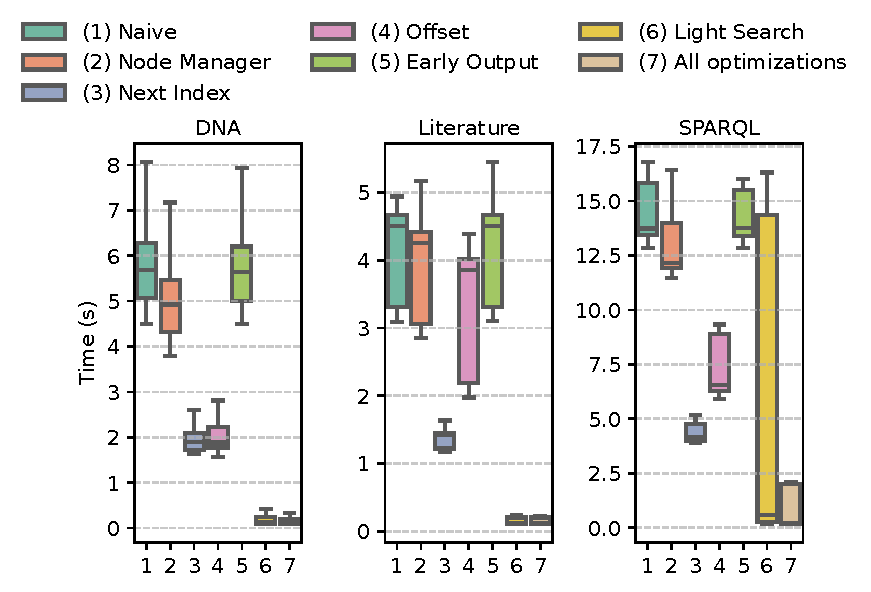
\includegraphics[width=.8\textwidth]{figures/versions-time.pdf}
	\caption{Runtime performance of \rematch\ optimizations}
	\label{fig:opt-time}
\end{figure}

\begin{figure}[t]
	\centering
	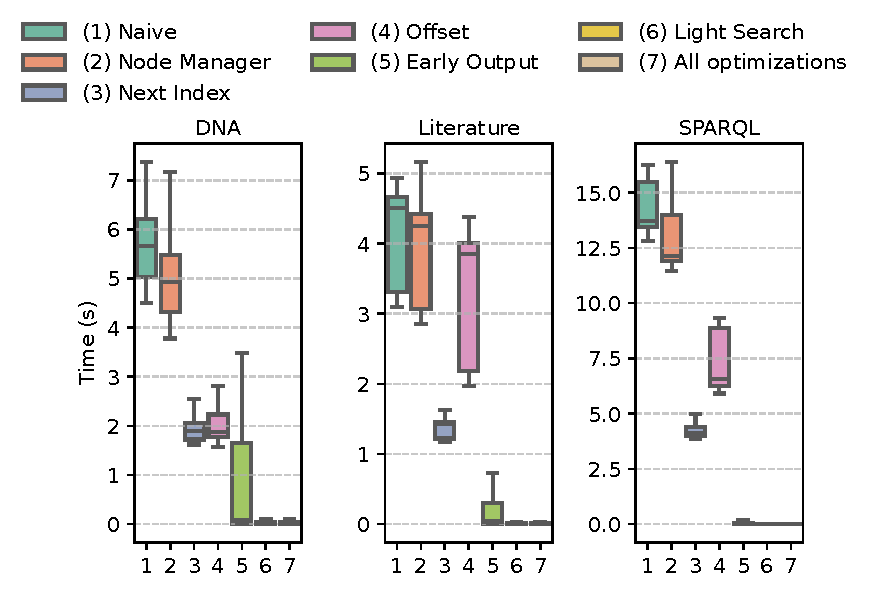
\includegraphics[width=.8\textwidth]{figures/versions-fot.pdf}
	\label{fig:opt-firstOT}
	\caption{Time to produce the first output of \rematch\ optimizations}
	\label{fig-optimizations}
\end{figure}

% TODO: Gonzalo says that Offset and Early Output worsen things. Asks if we
% tried to run Light Search without them.


\subsection{Discussion}
As we can observe (Figure~\ref{fig:opt-time}), each of our optimizations does
drop the total runtime of the workload when comparing against \textsc{Naive}.
The most consistent improvements come from \textsc{Next index} and
\textsc{Offset} optimizations. The \textsc{Light Search} version offers
significant improvements, particularly in the median, but bad cases can hamper
its performance, as witnessed over the \textsf{SPARQL} dataset. Over all the
dataset the full version of \rematch\ runs the fastest, as expected. Concerning
memory consumption (Table~\ref{tab-memory}) we first notice that the memory
consumption can vary considerably when considering the different datasets.
Notably, \textsf{DNA} demands more memory compared to \textsf{Literature} and
\textsf{SPARQL}. This for us seems to be related to the fact that the queries
are in general more complicated in that dataset, and they seem to negate the
improvements that some optimizations aim to give (notably \textsc{Offset} and
\textsc{Early Output}) . In terms of the different versions, \textsc{Node
Manager} drastically reduces memory usage, since this is its main purpose.
\textsc{Offset} and \textsc{Light Search} can also reduce memory usage, but
their performance varies significantly based on the query load. When it comes to
time to first output (Figure~\ref{fig-optimizations}), both \textsc{Early
Output} and \textsc{Light Search} show consistent and significant improvements,
as does \textsc{Next Index}. Over all the tested dimensions, the full version of
\rematch\ shows superior performance to any a single optimization on its own.
Slight hit in memory usage is noticeable in some cases due to the interaction of
different optimization methods in the full version, but overall memory usage is
still very low.


\begin{table}[t]
	\begin{tabular}{l|rrr}
		                      & \textsf{DNA} & \textsf{Literature} &
		                      \textsf{SPARQL} \\
		\hline
		\textsc{Naive}        & 823.30        & 379.90               & 1229.69
		\\
		\textsc{Node Manager} & 6.08         & 2.10                 & 8.75 \\
		\textsc{Next Index}   & 18.32        & 2.33                & 10.10 \\
		\textsc{Offset}       & 18.66        & 2.32                & 7.78 \\
		\textsc{Early Output} & 16.09        & 2.21                & 3.64 \\
		\textsc{Light Search} & 23.36        & 2.09                & 3.87
	\end{tabular}
	\caption{Average memory usage of \rematch\ versions (in MB).}
	\label{tab-memory}
\end{table}

\section{Comparison with other engines}\label{ss:comp}


\subsection{The setup}
Here we do a thorough analysis of how \rematch\ compares to classic RegEx
processing libraries. For a fair comparison, we considered a representative set
of RegEx engines implemented in C++ that can approximate the all-match semantics
using look-around operators. In addition, we also considered two engines that do
not support look-around operators; and will thus not output the same matches.
The engines used for comparison are:
\begin{itemize}
	\item \textsf{PCRE}~\citep{pcre} version: 8.45;
	\item \textsf{PCRE2}~\citep{pcre2} version 10.40 (using JPCRE2 C++
	wrapper~\citep{wrapper});
	\item \textsf{pcregrep}~\citep{grep} version 8.45;
	\item \textsf{Boost.Regex}~\citep{boost} version 1.81.0;
	\item \textsf{Oniguruma}~\citep{oniguruma} version 6.9.7.1;
	\item \textsf{RE2}~\citep{re2} version 2021--11--01; and
	\item \textsf{TRE}~\citep{tre} version 0.8.0.
\end{itemize}
For engines that support look-around operators (\textsf{PCRE}, \textsf{PCRE2},
\textsf{Boost} and \textsf{Oniguruma}) we rewrite the experiments from
Section~\ref{ss:setup} so that they retrieve all the matches. For \textsf{RE2}
and \textsf{TRE}, which do not support look-around operators, we rewrite the
queries using capture groups such they resemble as closely as possible the
original experiments, although they do not perform the same task. We also
include \textsf{grep} and use its PCRE syntax to have a standard command line
tool in our comparison. Notice that standard \textsf{grep} only allows matching
a single line to a pattern and not extracting any substring; thus an extended
version is used. Since standard \textsf{grep} does not allow extracting
substrings an extended version is used.


The results are presented in Figure~\ref{fig:comparison} and
Table~\ref{tab:outputs}. Here we compare only in terms of time. The memory
consumption was relatively stable along all the engines, with \rematch\ using
the most memory, but only by a negligible amount (kilobytes in our experiments),
which is justified by the extra bookkeeping done by \rematch\ in order to
retrieve all the matches.  \rematch\ had some spikes in memory usage for the
\textsf{DNA} dataset, and \textsf{PCRE2} in the \textsf{SPARQL} dataset, but the
document size still dominated memory usage significantly.

In this discussion, it is essential to recall that REmatch is incomparable with
standard RegEx engines, given that it uses a different query language for always
finding all matches (even DNA queries with look-around provide less number of
outputs). Then it is not our purpose here to prove that REmatch is ``faster''
than other RegEx engines. Quite the opposite, we want to test that, although
REmatch is running a more heavy processing task, the performance is comparable
to the standard and highly optimized RegEx engines.

\begin{table}
	\begin{tabular}{l|rrr}
		                   & \textsf{DNA}      & \textsf{Literature} &
		                   \textsf{SPARQL}   \\
		\hline
		\rematch           & \textbf{16,187.4} & \textbf{706.6}      &
		\textbf{29,424.2} \\
		\textsf{RE2}       & 10,556.9          & 704.9               & 12,287.8
		\\
		\textsf{PCRE}      & 13,130.4          & 705.1               &
		\textbf{29,424.2} \\
		\textsf{PCRE2}     & 13,130.4          & 705.1               &
		\textbf{29,424.2} \\
		\textsf{Boost}     & 13,130.4          & 642.6               &
		\textbf{29,424.2} \\
		\textsf{Oniguruma} & 13,130.4          & 705.5               &
		\textbf{29,424.2} \\
		\textsf{TRE}       & 10,556.9          & 704.2               & N/A
	\end{tabular}
	\caption{Average number of outputs (highest in bold).}
	\label{tab:outputs}
\end{table}

\begin{figure}[t]
	\centering
	\begin{subfigure}[b]{.8\textwidth}
		\centering
		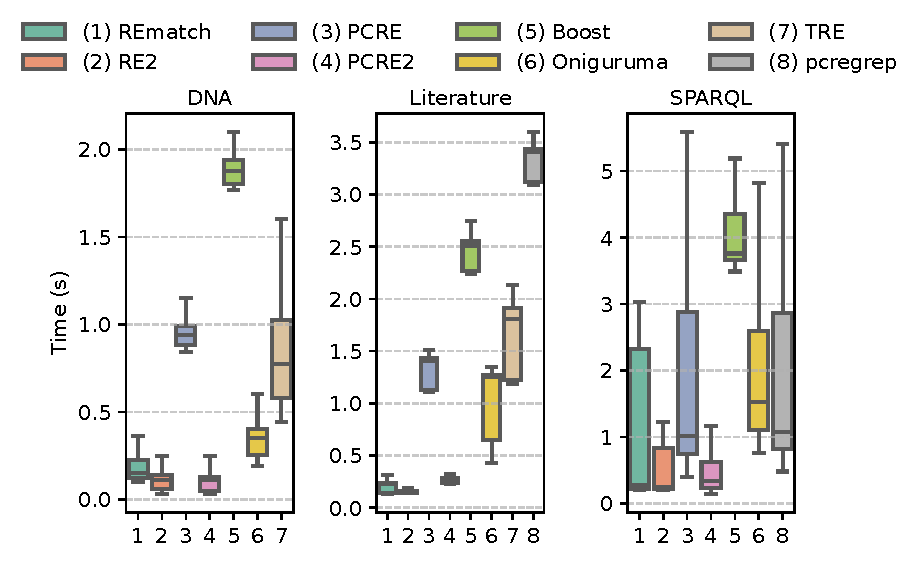
\includegraphics[width=\textwidth]{figures/lookahead-time.pdf}
	\end{subfigure}
	\caption{Runtime metrics of our experiments}
	\label{fig:comparison}
\end{figure}



\subsection{Discussion}
As we can see from Figure~\ref{fig:comparison}, \rematch\ shows good performance
as compared to other engines. On the \textsf{Literature} dataset, \rematch\ is
bested only by \textsf{RE2}, which does not look for all the outputs. On the
\textsf{DNA} dataset \rematch\ is a close third, bested only by \textsf{RE2} and
\textsf{PCRE2} by a tiny margin. When it comes to \textsf{SPARQL} the story is
similar, now with \textsf{pcregrep} also being fairly competitive. We remark
that on the \textsf{SPARQL} dataset \textsf{TRE} throws an error on every query,
while over the \textsf{DNA} dataset \textsf{pcregrep} runs out of buffer, since
the document is one very long line. Comparing the number of outputs, in
Table~\ref{tab:outputs} we can observe that \rematch\ generally does more work
compared to other engines. This is particularly evident when  comparing to
engines not using look-around operators (\textsf{RE2} and \textsf{TRE}). Even
for the engines with look-around supported, we sometimes cannot capture all the
outputs (for instance when two nested matches start at the same position), as
witnessed in Table~\ref{tab:outputs}. Interestingly, on the \textsf{SPARQL} set
of experiments look-ahead allows capturing all the outputs. While in this case
\textsf{PCRE2} does outperform \rematch\ in general, the median result for
\rematch\ is better, same as in the other two datasets. The bad cases for
\rematch\ come from the extra bookkeeping needed to assure that all matches will
be captured. Overall, the experiments illustrate that the task of encountering
\emph{all} the outputs  can be done with minimal overhead when comparing with
classical RegEx matching. 

\chapter[CONCLUSIONS]{Conclusions} \label{chpt:conclusions}
% !TeX root = ../Thesis.tex

In this thesis, we have meticulously analyzed the methods necessary to construct
an information extraction regex engine capable of supporting all-match
semantics, culminating in the development of the \texttt{REmatch} engine. A key
highlight is the use of enumeration algorithms as the fundamental framework,
notably the ECS data structure, which facilitates output-linear delay
enumeration. We have also implemented multiple optimizations to enhance the
engine's runtime efficiency and memory usage.

The \texttt{REmatch} engine proves to be a strong competitor against leading
regex engines, despite performing more complex tasks to ensure the extended
semantics not supported by other engines. The utility of all-match semantics, as
evidenced in our datasets, is particularly relevant in areas like DNA analysis
or linguistics, where overlapping matches are desirable in some contexts.

Future development plans must acknowledge that \texttt{REmatch} is not yet a
complete regex library for information extraction. Currently, the engine
requires more extensive testing and comprehensive documentation for it to be
able to participate in a in a production setting. In terms of performance
enhancements, several areas for optimization exist. For instance, the existing
\textit{all-match} algorithm does not feature parallel processing, a
modification that could significantly boost runtime efficiency. Additionally,
the potential expansion of the REQL query language to include more operators and
semantics is an exciting prospect. A notable improvement could be the relaxation
of constraints in REQL queries, allowing for captures under quantifier operators
(\texttt{*}, \texttt{+}, \texttt{?}, \texttt{\{n,m\}}). This adjustment would
allow a variable to correspond to multiple spans, providing increased
versatility in applications such as extracting multiple values from rows in CSV
files.


%%%%%%%%%%%%%
%       REFERENCES        %
%%%%%%%%%%%%%

\cleardoublepage
\phantomsection \label{references}
\bibliographystyle{apacite}
\renewcommand{\bibname}{REFERENCES}
\bibliography{references}

%%%%%%%%%%%%
%      APPENDICES      %
%%%%%%%%%%%%

\appendix % It is like a chapter, so each appendix (A, B, C...) must to be considered as a section

\newpage
\section{Proof of proposition \ref{prop:logicalVA}} \label{app:logicalVA}
Let $\texttt{e}$ be a REQL. We'll show that it there exists an $\varepsilon$-LogicalVA $\cA$ such that $\sem{\texttt{e}}_d = \sem{\cA}_d$ over any document $d$.  We proceed by induction. For each of the base cases shown in Table \ref*{tab-semantics} we can construct a LogicalVA $\cA$ with two states, one initial and one accepting, and with a single transition labeled as the char class equivalent to $\texttt{e}$ from the initial state to the accepting state. Is easy to see that this LogicalVA $\cA$ satisfies $\sem{\texttt{e}}_d = \sem{\cA}_d$ over any document $d$.

The inductive case goes as follows: without any loss of generality suppose that $\texttt{e}_1$ and $\texttt{e}_2$ are two REQLs such that there exists $\cA_1 = (Q_1, \delta_1, q_0^1, q_f^1)$ and $\cA_2 = (Q_2, \delta_2, q_0^2, q_f^2)$ both LogicalVAs that satisfy $\sem{\texttt{e}_1}_d = \sem{\cA_1}_d$ and  $\sem{\texttt{e}_2}_d = \sem{\cA_2}_d$ over any document $d$. Then, 

\begin{itemize}
    \item For $\texttt{e} = \texttt{e}_1\texttt{e}_2$ the LogicalVA $\cA = (Q_1 \cup Q_2, \delta_1 \cup \delta_2 \cup \{(q_f^1, \varepsilon, q_0^2)\}, q_0^1, q_f^2)$ is such that over any document $d$, $\sem{\texttt{e}}_d = \sem{\cA}_d$.
    \item For $\texttt{e} = \texttt{e}_1\texttt{|}\texttt{e}_2$ the LogicalVA $\cA = (Q_1 \cup Q_2 \cup \{q_0, q_f\}, \delta_1 \cup \delta_2 \cup \{(q_0, \varepsilon, q_0^1), (q_0, \varepsilon, q_0^2), (q_f^1, \varepsilon, q_f), (q_f^2, \varepsilon, q_f) \}, q_0, q_f^2)$ is such that over any document $d$, $\sem{\texttt{e}}_d = \sem{\cA}_d$.
    \item For $\texttt{e} = \texttt{!x\{}\texttt{e}_1\texttt{\}}$ the LogicalVA $\cA_\texttt{e} = (Q' \cup \{q_0, q_f\}, \delta' \cup \{(q_0, [x, q_0'), (q_f', x\rangle, q_f)\}, q_0, q_f)$ is such that over any document $d$, $\sem{\texttt{e}}_d = \sem{\cA_\texttt{e}}_d$.
    \item For $\texttt{e} = \texttt{e}_1\texttt{*}$ the LogicalVA $\cA = (Q_1, \delta_1 \cup \{(q_0^1, \varepsilon, q_f^1), (q_f^1, \varepsilon, q_0^1)\}, q_0^1, q_f^1)$ is such that over any document $d$, $\sem{\texttt{e}}_d = \sem{\cA}_d$.
    \item For $\texttt{e} = \texttt{e}_1\texttt{?}$ the LogicalVA $\cA = (Q_1, \delta_1 \cup \{(q_0^1, \varepsilon, q_f^1)\}, q_0^1, q_f^1)$ is such that over any document $d$, $\sem{\texttt{e}}_d = \sem{\cA}_d$.
    \item For $\texttt{e} = \texttt{e}_1\texttt{+}$ the LogicalVA $\cA = (Q_1, \delta_1 \cup \{(q_f^1, \varepsilon, q_0^1)\}, q_0^1, q_f^1)$ is such that over any document $d$, $\sem{\texttt{e}}_d = \sem{\cA}_d$.
    \item For $\texttt{e} = \texttt{e}_1\texttt{\{n,m\}}$ we can see that over any document $d$, $\sem{\texttt{e}}_d = \sem{(\texttt{e}_1)^n(\texttt{e}_1\texttt{?})^{m-n}}_d$ which can be easily shown to have an equivalent LogicalVA by applying induction with the previous rules.
\end{itemize}

\newpage
\section{Offset optimization} \label{app:offset}
% !TeX root = ../Thesis.tex

In some cases, opening a variable can be postponed in order to avoid the storage
of the information about runs that will not result in an output. To illustrate
this, consider the expression
\begin{center}
	\texttt{!x\{sparql[\textasciicircum \textbackslash n]*\}\textbackslash n}
\end{center}
which looks for the keyword \texttt{sparql}, and then proceeds to capture the
text until the first end of line symbol is reached. In a log file, such as the
ones studied in~\citet{AMRV16}, this roughly corresponds to capturing a SPARQL
query. Notice that here Algorithm \ref{alg:evaluation} would store the position
information for the opening of a variable \texttt{x} every time an \texttt{s}
would be read. If the document we are reading has the text \texttt{sparx}, this
run would then be extended for three more steps, although it will eventually be
abandoned, and not result in any outputs. Given the node management required
when changing the state of the ECS structure, this can bring a significant
overhead to evaluation. In cases such as these, we can actually postpone (i.e.,
offset) the opening of the variable \texttt{x} by proceeding as follows: (i)
first read the word \texttt{sparql}; (ii) now open a variable \texttt{x}, but
remember that it was actually opened six symbols before (i.e. it has an offset
6); (iii) proceed until the end of the expression. Then, when reconstructing the
output in case of a successful run, we will simply start reading the output six
symbols before the position that is actually stored in \texttt{ds} from
Algorithm \ref{alg:evaluation}. Intuitively, one could write the expression
above as:
\begin{center}
	\texttt{sparql!x\{$^{-6}$[\textasciicircum \textbackslash n]*\}
	\textbackslash n} 
\end{center}
in order to signal that when opened, the variable \texttt{x} actually stores
characters starting six positions before the guarded position.

\subsection{Offset logical VA} 
To formalize this concept we extend the definition of a logical VA as follows: a
\emph{logical variable-set automata} (offset logical VA) $\cAoff$ is a tuple
$(Q, \delta, \tau, q_0, q_f)$ that has the same structure as a logical VA, with
the addition of an \emph{offset marker} function $\tau$ that takes a variable
marker as input and returns an integer.

A configuration, a run and an accepting run of $\cAoff$ are defined exactly as
if $\cAoff$ were a logical VA. The only change is in the definition of its
semantics. Suppose that 
$$
	\rho \ = \ (q_0, i_0) \ \trans{o_1} \ (q_1, i_1) \ \trans{o_2} \ \cdots \ \trans{o_m} \ (q_m, i_m)
$$
is an accepting run of $\cAoff$. The mapping $\mu^\rho$ then is such that it
maps $x$ to $[i_j, i_k\rangle$ if, and only if, $o_{i_j + \tau([x)} = [x$ and
$o_{i_k + \tau(x\rangle)} = x\rangle$. In other words, the mapping $\mu^\rho$
acts in the same way as if $\cAoff$ were a logical VA, but taking into account
the offsets given by $\tau$ for each of the variable markers present in the
transitions of $\cAoff$. Therefore, the semantics of $\sem{\cAoff}_d$ of
$\cAoff$ over a document $d$ is defined as the set of all $\mu^\rho$ where
$\rho$ is an accepting run of $\cAoff$ over $d$.

Given the way Algorithm \ref*{alg:evaluation} works, it is desirable to be able
to construct an offset logical VA $\cAoff$ from an initial logical VA $\cA$ such
that: (i) the semantics are preserved, i.e., $\sem{\cAoff}_d = \sem{\cA}_d$, and
(ii) the offset function $\tau$ of $\cAoff$ is optimal in the sense of
maximizing the absolute values of the offsets for the variable markers, so that
the decision of changing the state of the ECS is postponed as much as possible
while reading the document. In REmatch, this is done by the following algorithm,
which we call \texttt{offset}.

\subsection{Offset algorithm}
In the implementation of REmatch, the \texttt{offset} optimization is done in
the early stages of preprocessing the query. After the first parse of the
expression, REmatch will build an extended variable automaton (eVA) as described
in Section \ref{sec:extendedVA}.

First, for each variable opening we build a list of all the transitions that
open this variable, and we do the same for each variable closing. The variable
opening/closing is then offset in bulk, namely, either all of the transitions of
the form $\Open{x}$ (or $\Close{x}$) are moved at once (in order to preserve
consistency), or none is. Let \texttt{captureList} be a list of all capture
transitions opening or closing some variable (for instance, they are all of the
form $\Open{x}$). For a capture transition $p\ \longtrans{\Open{x}}\ q$ we wish
to see if there is also a transition $q\ \longtrans{a}\ r$, in order to
interchange the transition reading the letter $a$, and the one opening the
variable $x$. That is, we wish to achieve the following transformation in the
states of our eVA:
$$p\ \longtrans{\Open{x}}\ q\ \longtrans{a}\ r \ \ \ \ \ \Rightarrow \ \ \ \ \ \
\ p\ \longtrans{a}\ q\ \longtrans{\Open{x}}\ r$$


We will say that we can offset $\Open{x}$ if the following conditions hold for
every transition $p\ \longtrans{\Open{x}}\ q$ appearing in \texttt{captureList}
associated with $\Open{x}$:
\begin{enumerate}
	\item $q$ is not a final state;
	\item There are no transitions of the form $q\ \longtrans{\Open{y}}\ r$, or
	of the form $p'\ \longtrans{v}\ q$, with $v$ a variable marker, in the
	automaton; \label{item:offset-cond-2}
	\item There is at least one transition of the form $q\ \longtrans{a}\ r$;
	\item For all transitions $q\ \longtrans{a}\ r$, $q$ can not be reached from
	$r$; and
	\item For any other transition $p'\ \longtrans{\Open{x}}\ q'$, if we take
	any $q\ \longtrans{a}\ r$, then $q'$ is not reachable from $r$.
\end{enumerate}

The first condition prevents offsetting a variable that leads to an accepting
run. The second condition prevents manipulating a state which has multiple
capture transitions associated with it. The third condition assures we actually
have a transition to offset. Fourth transition makes sure that in case of moving
the $\Open{x}$ variable marker forward, we will not create any loops involving
this variable marker. Finally, the last condition ensures that moving one
$\Open{x}$ variable marker will not result in an inconsistent run involving
another such transition. This could, for instance, happen if we had both $p\
\longtrans{\Open{x}}\ q\ \longtrans{a}\ r$ and $p'\ \longtrans{\Open{x}}\ q'\
\longtrans{a}\ q$ in our automaton, since offsetting the first $\Open{x}$
transition would result in an automaton that has a run opening $x$ twice.

Given each such list \texttt{captureList} (for example for $\Open{x}$), we
manipulate each set of transitions $p\ \longtrans{\Open{x}}\ q\ \longtrans{a}\
r$, by switching the $\Open{x}$ and $a$ symbols (in reality, an auxiliary state
is created for this). The new \texttt{captureList} is then populated by adding
the transitions $q\ \longtrans{\Open{x}}\ r$ to it, and the process is repeated
as long as the newly created list satisfies the five conditions specified above.

Finally, we process the variable offsets by finding the reverse topological
order of all the capture transitions. Then we offset the variables in this order
so that we can move them as far forward as possible. To illustrate why this is
important, consider the automaton consisting of a single run as follows:
$$q_0\ \longtrans{\Open{x}}\ q_1\ \longtrans{a}\ q_2\ \longtrans{\Close{x}}\
q_3\ \longtrans{b}\ q4$$ If we were to first offset the $\Open{x}$ variable
marker, this would result in:
$$q_0\ \longtrans{a}\ q_1\ \longtrans{\Open{x}^{-1}}\ q_2\
\longtrans{\Close{x}}\ q_3\ \longtrans{b}\ q4.$$ Notice that $\Open{x}$ cannot
be not be further offset due to condition (ii) above. Then, if we offset
$\Close{x}$ we get: $$q_0\ \longtrans{a}\ q_1\ \longtrans{\Open{x}^{-1}}\ q_2\
\longtrans{b}\ q_3\ \longtrans{\Close{x}^{-1}}\ q4$$ Which is suboptimal as
$\Open{x}^{-1}$ can still be offset from its position. If instead the variables
are processed in reverse topological order, this results in:
$$q_0\ \longtrans{a}\ q_1\ \longtrans{b}\ q_2\ \longtrans{\Open{x}^{-2}}\ q_3\
\longtrans{\Close{x}^{-1}}\ q4$$ which is better in terms of the maximization of
the absolute values of the offsets.

\newpage
\section{Proof of theorem \ref{theo:segmentation}} \label{app:segmentation}
% !TeX root = ../Thesis.tex

\begin{proof}
	Let us name the sequence as $\sigma = [i_1, j_1\rangle, \ldots, [i_k,
	j_k\rangle$. It not hard to see that $\sigma$ is a segmentation. First
	notice that $i$ and $j$ can only change their values to $\ell$ and $\ell +
	1$ in the execution, so as $ 0 \leq \ell \leq n$, then every span in
	$\sigma$ must be contained in the document. Now suppose that $k > 1$
	(otherwise $\sigma$ is trivially a segmentation). Pick any $1 \leq h < k$.
	Then Algorithm \ref*{alg:segmentation} adds the span $\sspan{i_h, j_h}$ in
	line 10 after an $\textbf{else if}$ statement that ensures that $j_h \leq
	\ell$ in that iteration. Rightly afterwards on line 11 $i$ starts holding
	the value $\ell + 1$, then $j_h < i$ right at the end of that iteration. So
	whenever the algorithm outputs $[i_{h+1}, j_{h+1}\rangle$ it is certain that
	$j_h < i_{h+1}$ because $i$ cannot decrease in value. 

    Let us prove now that $\sigma$ is a valid segmentation. Let $\mu \in
    \sem{\cA}_d$ be a mapping of $\cA$ over $d$. We must show that there exists
    $1 \leq h \leq k$ such that there is a mapping $\mu' \in
    \sem{\cA}(d\sspan{i_h, j_h})$ that satisfies $\mu = \mu'_{+h}$. As we have
    the mapping $\mu$ then there is an accepting run 
    $$
    \rho \ = \ (q_0, \iota_0) \ \trans{o_1} \ (q_1, \iota_1) \ \trans{o_2} \ \cdots \ \trans{o_m} \ (q_m, \iota_m)
    $$ 
    over $d$ that satisfies $q_m = q_f$ and such that the spans that $\mu$ holds
    are all contained inside the span $\sspan{\iota_0, \iota_m}$. We proceed to
    show that the span $\sspan{\iota_0, \iota_m}$ must be contained inside a
    span $\sspan{i_h, j_h}$ of $\sigma$. In Algorithm \ref{alg:segmentation},
    consider the iteration inside the loop when $\ell = \iota_0$. We can be sure
    that in the iteration the function $\texttt{next}_\delta(S, a_\ell)$ does
    not return \texttt{ends} as true, because we know that $\rho$ is accepting
    and it doesn't end at $\iota_0$. Therefore the variable $i$ does not change
    its value and it must satisfy that $i \leq \iota_0$ at the end of this
    iteration. The same argument can be made for the iterations that follow,
    namely when $\ell$ takes the values $\iota_1, \ldots, \iota_{m-1}$, the
    variable $i$ must satisfy $i \leq \iota_0$ at the end of each of these
    iterations. Now consider the iteration when $\ell = \iota_m$. It is clear
    that $\texttt{next}_\delta(S, a_\ell)$ will return \texttt{outputs} as true
    because $\rho$ is accepting. Hence, $j$ will change its value to $\iota_m +
    1$ in this iteration, Thus $j < \iota_m$. Given that the mapping $\mu$
    cannot contain a zero-length span (otherwise $\cA$ would not constitute a
    valid logical VA), then $i \leq \iota_0 < \iota_m \leq j$. In future
    iterations is easy to see that:
    \begin{enumerate}
        \item[(i)] the value of $j$ can only increase,
        \item[(ii)] the value of $i$ can cannot change before outputting a span,
        and
        \item[(iii)] the algorithm will eventually output a span $\sspan{i_h,
        j_h}$ that satisfies $i_h \leq \iota_0 < \iota_m \leq j_h$. 
    \end{enumerate}
    Therefore, $\sspan{\iota_0, \iota_m}$ is contained inside a span
    $\sspan{i_h, j_h}$ of $\sigma$. Now if we take the document $d\sspan{i_h,
    j_h}$ it must hold that there is a mapping $\mu' \sem{\cA}(d\sspan{i_h,
    j_h})$ defined by the accepting run 
    $$
    \rho' \ = \ (q_0, \iota_0-h) \ \trans{o_1} \ (q_1, \iota_1-h) \ \trans{o_2} \ \cdots \ \trans{o_m} \ (q_m, \iota_m-h)
    $$ 
    of $\cA$ over $d\sspan{i_h, j_h}$. Furthermore, it satisfies that $\mu =
    \mu'_{+h}$.

    The converse is straightforward. Let $\mu' \in \sem{\cA}(d\sspan{i_h, j_h})$
    be a mapping of $\cA$ over $d\sspan{i_h, j_h}$ for some $1 \leq h \leq k$.
    Therefore, there exists an accepting run
    $$
    \rho' \ = \ (q_0, \iota_0) \ \trans{o_1} \ (q_1, \iota_1) \ \trans{o_2} \ \cdots \ \trans{o_m} \ (q_f, \iota_m)
    $$
    of $\cA$ over $d\sspan{i_h, j_h}$. This means that it must exist an
    accepting run
    $$
    \rho \ = \ (q_0, \iota_0+h) \ \trans{o_1} \ (q_1, \iota_1+h) \ \trans{o_2} \ \cdots \ \trans{o_m} \ (q_f, \iota_m+h)
    $$
    of $\cA$ over $d$. It is straightforward that the mapping $\mu^\rho$ is the
    same mapping $\mu'$ with an offset, i.e. $\mu^\rho = \mu'_{+h}$. Thus,
    $\mu'_{+h} \in \sem{\cA}_d$. \qedhere 
    

\end{proof}

\end{document}
